%%
% Copyright (c) 2017 - 2019, Pascal Wagler;  
% Copyright (c) 2014 - 2019, John MacFarlane
% 
% All rights reserved.
% 
% Redistribution and use in source and binary forms, with or without 
% modification, are permitted provided that the following conditions 
% are met:
% 
% - Redistributions of source code must retain the above copyright 
% notice, this list of conditions and the following disclaimer.
% 
% - Redistributions in binary form must reproduce the above copyright 
% notice, this list of conditions and the following disclaimer in the 
% documentation and/or other materials provided with the distribution.
% 
% - Neither the name of John MacFarlane nor the names of other 
% contributors may be used to endorse or promote products derived 
% from this software without specific prior written permission.
% 
% THIS SOFTWARE IS PROVIDED BY THE COPYRIGHT HOLDERS AND CONTRIBUTORS 
% "AS IS" AND ANY EXPRESS OR IMPLIED WARRANTIES, INCLUDING, BUT NOT 
% LIMITED TO, THE IMPLIED WARRANTIES OF MERCHANTABILITY AND FITNESS 
% FOR A PARTICULAR PURPOSE ARE DISCLAIMED. IN NO EVENT SHALL THE 
% COPYRIGHT OWNER OR CONTRIBUTORS BE LIABLE FOR ANY DIRECT, INDIRECT, 
% INCIDENTAL, SPECIAL, EXEMPLARY, OR CONSEQUENTIAL DAMAGES (INCLUDING,
% BUT NOT LIMITED TO, PROCUREMENT OF SUBSTITUTE GOODS OR SERVICES; 
% LOSS OF USE, DATA, OR PROFITS; OR BUSINESS INTERRUPTION) HOWEVER 
% CAUSED AND ON ANY THEORY OF LIABILITY, WHETHER IN CONTRACT, STRICT 
% LIABILITY, OR TORT (INCLUDING NEGLIGENCE OR OTHERWISE) ARISING IN 
% ANY WAY OUT OF THE USE OF THIS SOFTWARE, EVEN IF ADVISED OF THE 
% POSSIBILITY OF SUCH DAMAGE.
%%

%%
% For usage information and examples visit the GitHub page of this template:
% https://github.com/Wandmalfarbe/pandoc-latex-template
%%

\PassOptionsToPackage{unicode=true}{hyperref} % options for packages loaded elsewhere
\PassOptionsToPackage{hyphens}{url}
\PassOptionsToPackage{dvipsnames,svgnames*,x11names*,table}{xcolor}
%
\documentclass[
  a4paper,
,tablecaptionabove
]{scrbook}
\usepackage{lmodern}
\usepackage{setspace}
\setstretch{1.2}
\usepackage{amssymb,amsmath}
\usepackage{ifxetex,ifluatex}
\ifnum 0\ifxetex 1\fi\ifluatex 1\fi=0 % if pdftex
  \usepackage[T1]{fontenc}
  \usepackage[utf8]{inputenc}
  \usepackage{textcomp} % provides euro and other symbols
\else % if luatex or xelatex
  \usepackage{unicode-math}
  \defaultfontfeatures{Scale=MatchLowercase}
  \defaultfontfeatures[\rmfamily]{Ligatures=TeX,Scale=1}
\fi
% use upquote if available, for straight quotes in verbatim environments
\IfFileExists{upquote.sty}{\usepackage{upquote}}{}
\IfFileExists{microtype.sty}{% use microtype if available
  \usepackage[]{microtype}
  \UseMicrotypeSet[protrusion]{basicmath} % disable protrusion for tt fonts
}{}
\makeatletter
\@ifundefined{KOMAClassName}{% if non-KOMA class
  \IfFileExists{parskip.sty}{%
    \usepackage{parskip}
  }{% else
    \setlength{\parindent}{0pt}
    \setlength{\parskip}{6pt plus 2pt minus 1pt}}
}{% if KOMA class
  \KOMAoptions{parskip=half}}
\makeatother
\usepackage{xcolor}
\definecolor{default-linkcolor}{HTML}{A50000}
\definecolor{default-filecolor}{HTML}{A50000}
\definecolor{default-citecolor}{HTML}{4077C0}
\definecolor{default-urlcolor}{HTML}{4077C0}
\IfFileExists{xurl.sty}{\usepackage{xurl}}{} % add URL line breaks if available
\IfFileExists{bookmark.sty}{\usepackage{bookmark}}{\usepackage{hyperref}}
\hypersetup{
  pdftitle={Embedded Wizard tutorial},
  pdfauthor={Andreas Deininger},
  pdfkeywords={Embedded Wizard Tutorial},
  pdfborder={0 0 0},
  breaklinks=true}
\urlstyle{same}  % don't use monospace font for urls
\usepackage[margin=2.5cm,includehead=true,includefoot=true,centering]{geometry}
\usepackage{longtable,booktabs}
% Allow footnotes in longtable head/foot
\IfFileExists{footnotehyper.sty}{\usepackage{footnotehyper}}{\usepackage{footnote}}
\makesavenoteenv{longtable}
\usepackage{graphicx,grffile}
\makeatletter
\def\maxwidth{\ifdim\Gin@nat@width>\linewidth\linewidth\else\Gin@nat@width\fi}
\def\maxheight{\ifdim\Gin@nat@height>\textheight\textheight\else\Gin@nat@height\fi}
\makeatother
% Scale images if necessary, so that they will not overflow the page
% margins by default, and it is still possible to overwrite the defaults
% using explicit options in \includegraphics[width, height, ...]{}
\setkeys{Gin}{width=\maxwidth,height=\maxheight,keepaspectratio}
\setlength{\emergencystretch}{3em}  % prevent overfull lines
\providecommand{\tightlist}{%
  \setlength{\itemsep}{0pt}\setlength{\parskip}{0pt}}
\setcounter{secnumdepth}{5}
% Redefines (sub)paragraphs to behave more like sections
\ifx\paragraph\undefined\else
  \let\oldparagraph\paragraph
  \renewcommand{\paragraph}[1]{\oldparagraph{#1}\mbox{}}
\fi
\ifx\subparagraph\undefined\else
  \let\oldsubparagraph\subparagraph
  \renewcommand{\subparagraph}[1]{\oldsubparagraph{#1}\mbox{}}
\fi

% Make use of float-package and set default placement for figures to H
\usepackage{float}
\floatplacement{figure}{H}


\title{Embedded Wizard tutorial}
\author{Andreas Deininger <andreas@deininger.net>}
\date{2019-03-16}





%%
%% added
%%

%
% No language specified? take American English.
%

\ifnum 0\ifxetex 1\fi\ifluatex 1\fi=0 % if pdftex
  \usepackage[shorthands=off,main=english]{babel}
\else
    % See issue https://github.com/reutenauer/polyglossia/issues/127
  \renewcommand*\familydefault{\sfdefault}
    % load polyglossia as late as possible as it *could* call bidi if RTL lang (e.g. Hebrew or Arabic)
  \usepackage{polyglossia}
  \setmainlanguage[]{english}
\fi


%
% colors
%
\usepackage[]{xcolor}

%
% listing colors
%
\definecolor{listing-background}{HTML}{F7F7F7}
\definecolor{listing-rule}{HTML}{B3B2B3}
\definecolor{listing-numbers}{HTML}{B3B2B3}
\definecolor{listing-text-color}{HTML}{000000}
\definecolor{listing-keyword}{HTML}{435489}
\definecolor{listing-identifier}{HTML}{435489}
\definecolor{listing-string}{HTML}{00999A}
\definecolor{listing-comment}{HTML}{8E8E8E}
\definecolor{listing-javadoc-comment}{HTML}{006CA9}

%\definecolor{listing-background}{rgb}{0.97,0.97,0.97}
%\definecolor{listing-rule}{HTML}{B3B2B3}
%\definecolor{listing-numbers}{HTML}{B3B2B3}
%\definecolor{listing-text-color}{HTML}{000000}
%\definecolor{listing-keyword}{HTML}{D8006B}
%\definecolor{listing-identifier}{HTML}{000000}
%\definecolor{listing-string}{HTML}{006CA9}
%\definecolor{listing-comment}{rgb}{0.25,0.5,0.35}
%\definecolor{listing-javadoc-comment}{HTML}{006CA9}

%
% for the background color of the title page
%
\usepackage{pagecolor}
\usepackage{afterpage}

%
% TOC depth and 
% section numbering depth
%
\setcounter{tocdepth}{3}
\setcounter{secnumdepth}{3}

%
% break urls
%
\PassOptionsToPackage{hyphens}{url}

%
% When using babel or polyglossia with biblatex, loading csquotes is recommended 
% to ensure that quoted texts are typeset according to the rules of your main language.
%
\usepackage{csquotes}

%
% captions
%
\definecolor{caption-color}{HTML}{777777}
\usepackage[font={stretch=1.2}, textfont={color=caption-color}, position=top, skip=4mm, labelfont=bf, singlelinecheck=false, justification=raggedright]{caption}
\setcapindent{0em}
\captionsetup[longtable]{position=above}

%
% blockquote
%
\definecolor{blockquote-border}{RGB}{221,221,221}
\definecolor{blockquote-text}{RGB}{119,119,119}
\usepackage{mdframed}
\newmdenv[rightline=false,bottomline=false,topline=false,linewidth=3pt,linecolor=blockquote-border,skipabove=\parskip]{customblockquote}
\renewenvironment{quote}{\begin{customblockquote}\list{}{\rightmargin=0em\leftmargin=0em}%
\item\relax\color{blockquote-text}\ignorespaces}{\unskip\unskip\endlist\end{customblockquote}}

%
% Source Sans Pro as the de­fault font fam­ily
% Source Code Pro for monospace text
%
% 'default' option sets the default 
% font family to Source Sans Pro, not \sfdefault.
%
\usepackage[default]{sourcesanspro}
\usepackage{sourcecodepro}

% XeLaTeX specific adjustments for straight quotes: https://tex.stackexchange.com/a/354887
% This issue is already fixed (see https://github.com/silkeh/latex-sourcecodepro/pull/5) but the 
% fix is still unreleased.
% TODO: Remove this workaround when the new version of sourcecodepro is reelased on CTAN.
\ifxetex
\makeatletter
\defaultfontfeatures[\ttfamily]
  { Numbers   = \sourcecodepro@figurestyle,
    Scale     = \SourceCodePro@scale,
    Extension = .otf }
\setmonofont
  [ UprightFont    = *-\sourcecodepro@regstyle,
    ItalicFont     = *-\sourcecodepro@regstyle It,
    BoldFont       = *-\sourcecodepro@boldstyle,
    BoldItalicFont = *-\sourcecodepro@boldstyle It ]
  {SourceCodePro}
\makeatother
\fi

%
% heading color
%
\definecolor{heading-color}{RGB}{40,40,40}
\addtokomafont{section}{\color{heading-color}}
% When using the classes report, scrreprt, book, 
% scrbook or memoir, uncomment the following line.
%\addtokomafont{chapter}{\color{heading-color}}

%
% variables for title and author
%
\usepackage{titling}
\title{Embedded Wizard tutorial}
\author{Andreas Deininger <andreas@deininger.net>}

%
% tables
%

\definecolor{table-row-color}{HTML}{F5F5F5}
\definecolor{table-rule-color}{HTML}{999999}

%\arrayrulecolor{black!40}
\arrayrulecolor{table-rule-color}     % color of \toprule, \midrule, \bottomrule
\setlength\heavyrulewidth{0.3ex}      % thickness of \toprule, \bottomrule
\renewcommand{\arraystretch}{1.3}     % spacing (padding)

% Reset rownum counter so that each table
% starts with the same row colors.
% https://tex.stackexchange.com/questions/170637/restarting-rowcolors
\let\oldlongtable\longtable
\let\endoldlongtable\endlongtable
\renewenvironment{longtable}{
\rowcolors{3}{}{table-row-color!100}  % row color
\oldlongtable} {
\endoldlongtable
\global\rownum=0\relax}

% Unfortunately the colored cells extend beyond the edge of the 
% table because pandoc uses @-expressions (@{}) like so: 
%
% \begin{longtable}[]{@{}ll@{}}
% \end{longtable}
%
% https://en.wikibooks.org/wiki/LaTeX/Tables#.40-expressions

%
% remove paragraph indention
%
\setlength{\parindent}{0pt}
\setlength{\parskip}{6pt plus 2pt minus 1pt}
\setlength{\emergencystretch}{3em}  % prevent overfull lines

%
%
% Listings
%
%


%
% header and footer
%
\usepackage{fancyhdr}

\fancypagestyle{eisvogel-header-footer}{
  \fancyhead{}
  \fancyfoot{}
  \lhead[Embedded Wizard tutorial]{}
  \chead[]{}
  \rhead[]{}
  \lfoot[\thepage]{}
  \cfoot[]{}
  \rfoot[]{\thepage}
  \renewcommand{\headrulewidth}{0.4pt}
  \renewcommand{\footrulewidth}{0.4pt}
}
\pagestyle{eisvogel-header-footer}

%%
%% end added
%%

\begin{document}

%%
%% begin titlepage
%%

\begin{titlepage}
\newgeometry{left=6cm}
\newcommand{\colorRule}[3][black]{\textcolor[HTML]{#1}{\rule{#2}{#3}}}
\begin{flushleft}
\noindent
\\[-1em]
\color[HTML]{5F5F5F}
\makebox[0pt][l]{\colorRule[435488]{1.3\textwidth}{4pt}}
\par
\noindent

{ \setstretch{1.4}
\vfill
\noindent {\huge \textbf{\textsf{Embedded Wizard tutorial}}}
\vskip 2em
\noindent
{\Large \textsf{Andreas Deininger}
\vskip -3mm
\noindent {\large \textit{andreas@deininger.net}}
\vfill
}


\textsf{2019-03-16}}
\end{flushleft}
\end{titlepage}
\restoregeometry

%%
%% end titlepage
%%

{
\setcounter{tocdepth}{3}
\tableofcontents
}

\chapter{Introduction}

\rhead[]{Introduction}

\hypertarget{_about_embedded_wizard}{%
\section{About Embedded Wizard}
\label{_about_embedded_wizard}}

\href{https://www.embedded-wizard.de/}{Embedded Wizard} is a graphical
user interface tool developed and distributed by
\href{https://www.tara-systems.de/}{TARA Systems GmbH} for creating
graphical user interface (GUI) applications mainly for embedded systems.

\hypertarget{_motivation_for_this_tutorial}{%
\section{Motivation for this
tutorial}\label{_motivation_for_this_tutorial}}

At work, we used Embedded Wizard GUI builder extensively in a
development project. While the Embedded Wizard software proved to be an
extremely powerful tool, getting started with this tool was quite
challenging for us:

\begin{itemize}
\item
  Embedded Wizard strictly follows and implements an object oriented
  programming approach. These concepts may not be immediately obvious to
  a novice user however, who may be overwhelmed by terminology of
  properties, outlets, class variants, property references and so on.
\item
  Device integration will an essential part of every real world project,
  this is where newbies are often struggling. This situation is worsened
  by the fact that Embedded Wizards supports a broad range of target
  devices, each one being different, which makes it hard to provide
  universal instructions here.
\item
  Embedded Wizard comes with a comprehensive, excellent
  \href{http://doc.embedded-wizard.de}{documentation} which covers all
  aspects of the system. This documentation is topic oriented and even
  comes with several small, helpful sample projects. However, it remains
  a challenge to gain understanding on how to use and properly connect
  these code snippets in the context of a bigger application.
\end{itemize}

By time, we get acquainted to Embedded Wizard and the underlying
concepts, the learning curve was pretty steep though. At that time, I
sorely missed a step-by step tutorial, explaining in detail the
development of a reasonably small, but already meaningful application.
Since I couldn't find anything like that I took the initiative and
started authoring such a tutorial by myself. Hopefully the provided
tutorial will be helpful for you and will get you started with Embedded
Wizard trouble-free and quickly!

\hypertarget{_scope_of_the_tutorial}{%
\section{Scope of the tutorial}\label{_scope_of_the_tutorial}}

This project aims at providing a tutorial for potential users of
Embedded Wizard to get them started quickly.

While building a sample application step by step, the tutorial covers
the following topics:

\begin{itemize}
\item
  \href{https://deining.github.io/EmWiTutorial/EmWiTutorial/latest/HelloWorld.html}{Basic
  steps when building a GUI application}
\item
  \href{https://deining.github.io/EmWiTutorial/EmWiTutorial/latest/ComponentReusability.html}{Developing
  and prototyping reusable graphical components}
\item
  \href{https://deining.github.io/EmWiTutorial/EmWiTutorial/latest/DeviceIntegrationBrowser.html}{Device
  integration}
\item
  \href{https://deining.github.io/EmWiTutorial/EmWiTutorial/latest/LocalizingYourApplication.html}{Localization
  of your application}
\item
  Persistent data storage on the target device
\end{itemize}

\hypertarget{_sample_application}{%
\section{Sample application}\label{_sample_application}}

In the course of this tutorial, we are going to develop a small GUI
application for execution inside a web browser. A live preview of the
sample application is shown in
\protect\hyperlink{fig:TutorialApp}{figure\_title} below. Feel free to
click inside and explore the app and its features:

\begin{figure}
\centering
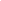
\includegraphics{./../asciidoc/modules/ROOT/assets/images/icons/1x1.png}
\caption{Tutorial application, live preview}
\end{figure}

The tutorial application comprises two components, titled \emph{Bell}
and \emph{Weather report}. When pressing the push-button of the
\emph{bell} component, a beep will sound. When pressing the push-button
of the \emph{weather report} component, you will be redirected to a web
site showing a weather report. The application is localized, by clicking
on a flag icon in the upper right corner you can select either
\emph{English} or German as language of the user interface. When running
the app in its own browser window, the chosen language setting will be
stored inside the local storage of your web browser and will be
remembered on the next reload or startup. This way you can keep your
language setting, even when you exit and restart your browser.

\hypertarget{_target_audience_prior_knowledge}{%
\section{Target audience, prior
knowledge}\label{_target_audience_prior_knowledge}}

The main audience for the book are professional developers that want
leverage Embedded Wizard platform when developing GUi applications for
their embedded devices. This tutorial assumes that you have experience
with one or more programming languages (C, C++, Java, C\#, \ldots​) and
that you are familiar with the concepts of object oriented programming.
In the first place, this tutorial wants to provide easy to follow step
by step instructions on how to build a small, but meaningful sample
application. Quite often, the tutorial goes beyond this and tries to
reveal the architectural patterns behind the application, specifically
pointing out how the patterns are implemented by Embedded wizard. While
doing so we assume at least limited familiarity with the patterns of
object oriented design, this tutorial does \textbf{not} explain things
like classes, methods, inheritance, \ldots​ from ground up.

\begin{quote}
\textbf{Important}

If you haven't written any code by hand, this tutorial is most likely
\textbf{not} for you. Don't be deceived: while Embedded Wizard provides
a graphical oriented programming approach in the first place, for any
meaningful application, you have to write code sooner or later to get
the desired results. Don't be scared, though: this isn't too hard,
everything will be explained in the course of this tutorial.
\end{quote}

\hypertarget{_prerequisites}{%
\section{Prerequisites}\label{_prerequisites}}

Download and install
\href{https://www.embedded-wizard.de/download/}{Embedded Wizard Free
Edition}, version 9.10. The free edition has all features of the
Professional edition, is is restricted to small projects however.
Luckily, the free edition allows to develop and to run the tutorial
application without limitation.

\hypertarget{_feedback_and_questions}{%
\section{Feedback and questions}\label{_feedback_and_questions}}

If you have any suggestion for improvement or comment concerning this
tutorial, feel free to open an
\href{https://github.com/deining/EmWiTutorial/issues}{issue} in the
github repository associated with this tutorial.

For general question unrelated to this tutorial, you may make use of the
\href{https://ask.embedded-wizard.de}{question and answer site} for
Embedded Wizard users and UI developers.

Let's get started with a simple
\href{https://deining.github.io/EmWiTutorial/EmWiTutorial/latest/HelloWorld.html}{Hello,
world} example!

\chapter{Getting started with 'Hello world'}

\rhead[]{Getting started with 'Hello world'}

For every language, its a good practice to start by printing out
\emph{Hello World!}. So let's start and do this with Embedded Wizard,
too!

\hypertarget{_setting_up_a_new_project}{%
\section{Setting up a new project}\label{_setting_up_a_new_project}}

\begin{enumerate}
\def\labelenumi{\arabic{enumi}.}
\item
  Start up Embedded Wizard Studio
\item
  From the main menu, select \textsc{Project > New \ldots}​ to start a
  new project
\item
  A popup appears:

  \begin{itemize}
  \item
    In the template, select the item {[}Empty project{]}.
  \item
    Specify \emph{EmWiTutorial} as project name.
  \item
    For the \emph{Location} of your project, specify a folder of your
    choice on your local file system.
  \end{itemize}
\item
  Once project name and location are set, press the button btn:{[}Create
  new project{]} to bring up the new project.
\end{enumerate}

\hypertarget{_structure_of_the_project}{%
\section{Structure of the project}\label{_structure_of_the_project}}

Let's have a look at the structure of the newly created project. As you
can see from \protect\hyperlink{fig:ProjectLayout}{figure\_title}, in
total 4 items were added to the main area, the so called
\href{https://doc.embedded-wizard.de/composer-window}{composer window}:

\begin{figure}
\centering
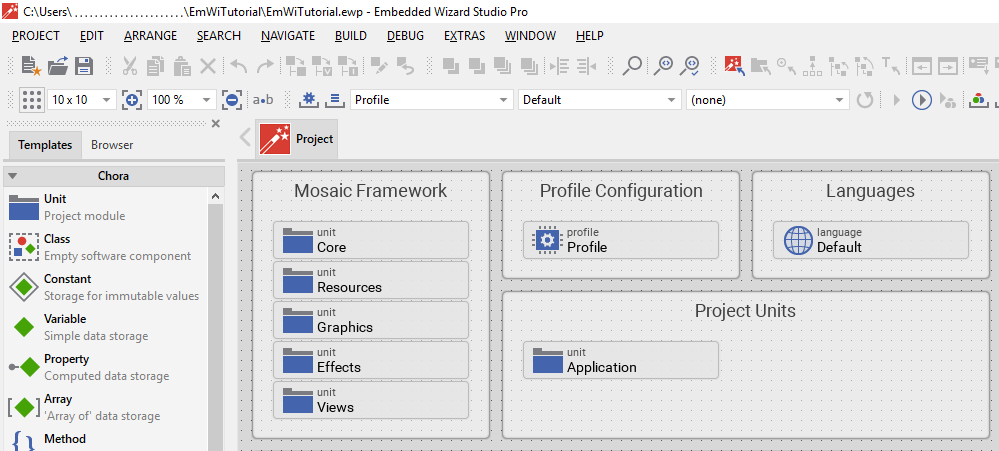
\includegraphics{./../asciidoc/modules/ROOT/assets/images/helloworld/InitialProject.png}
\caption{Inital project layout}
\end{figure}

These 4 groups serve totally different purposes:

\begin{description}
\item[Mosaic Framework]
This is embedded wizard's GUI framework used under the hood. You
shouldn't be concerned about this right now.
\item[Profile configuration]
A profile is used to store configuration parameters for your project. By
using different profiles, you can customize the project settings to the
different target(s) that you ant to use.
\item[Languages]
The concept of languages is deeply embedded into the system's language
\emph{Chora}. If you want to create a multi-lingual app, you can do so
by simply adding more languages here.
\item[Project units]
That's the most interesting part for now, so let's start explaining the
concept behind:
\end{description}

\hypertarget{_units}{%
\subsection{Units}\label{_units}}

\href{https://doc.embedded-wizard.de/unit-member}{Units} are a way to
structure your project. For now, we will deal with one unit only, the
\emph{Application} unit. While we use this unit for now, we will add
more units later on. Units are a kind of container for our components
used, so have a look now what's inside the \emph{Application} unit:

\begin{enumerate}
\def\labelenumi{\arabic{enumi}.}
\item
  Double click on the icon
  
\includegraphics{./../asciidoc/modules/ROOT/assets/images/icons/ApplicationUnitIcon.png},
  representing the \emph{Application} unit.
\item
  Inside the composer window, a second tab appears which shows the
  contents inside the unit which is now opened.
\end{enumerate}

The unit contains one single element only, the \emph{Application} class:

\begin{figure}
\centering
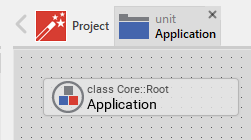
\includegraphics{./../asciidoc/modules/ROOT/assets/images/helloworld/ApplicationUnit.png}
\caption{Application unit with application class inside}
\end{figure}

\hypertarget{_application_class}{%
\subsection{Application class}\label{_application_class}}

The \emph{Application} class is the root element, standing at the very
top our application. Again let's see what's inside the
\emph{Application} class, which is a kind of container for the elements
of the class:

\begin{enumerate}
\def\labelenumi{\arabic{enumi}.}
\item
  Double click on the icon
  
\includegraphics{./../asciidoc/modules/ROOT/assets/images/icons/ApplicationClassIcon.png},
  representing the \emph{Application} class.
\item
  Inside the composer window, a third tab appears which shows the
  contents of the class which is now opened:
\end{enumerate}

\begin{figure}
\centering
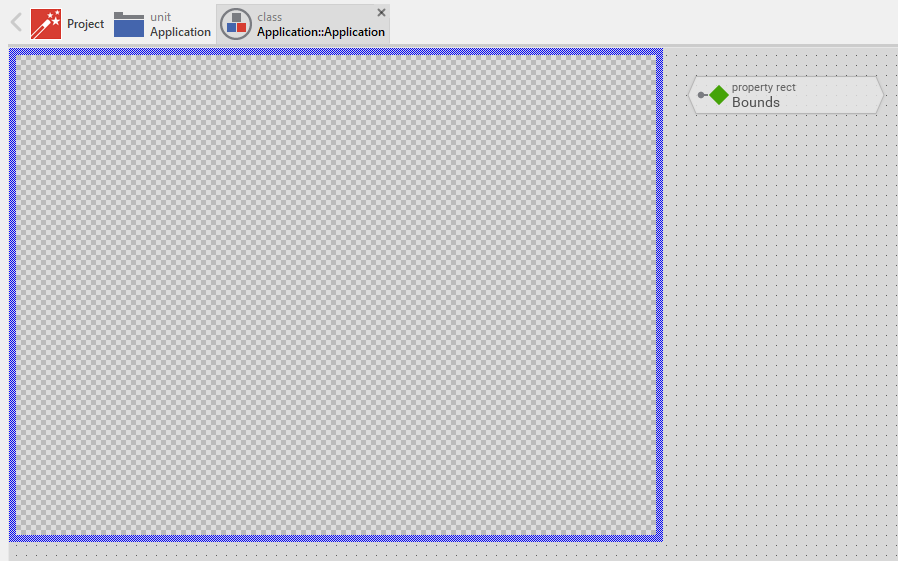
\includegraphics{./../asciidoc/modules/ROOT/assets/images/helloworld/ApplicationClass.png}
\caption{Application class with root canvas inside}
\end{figure}

All you will see here is the transparent root canvas, surrounded by a
blue border. That's not much, so let's put some text on the canvas:

\begin{itemize}
\item
  In the
  \href{https://doc.embedded-wizard.de/gallery-templates-window}{gallery
  templates window}, left to the main composer window, make sure that
  the tab \emph{Templates} is selected.
\item
  In the main area of the templates window, you will find several text
  item entries. Click on the item \emph{Views}, which will open and show
  all the \emph{view}-subitems (the items of the templates window
  follows are arranged in an accordion style layout).
\item
  Identify the item
  
\includegraphics{./../asciidoc/modules/ROOT/assets/images/icons/TextViewIcon.png}
  Text, representing a simple text view. Click on the element, drag it
  over to the root canvas and place it in the middle of the canvas.
\item
  If all went fine, you will see a tiny white text element labelled
  \emph{Text} in the middle of the canvas.
\end{itemize}

\begin{figure}
\centering
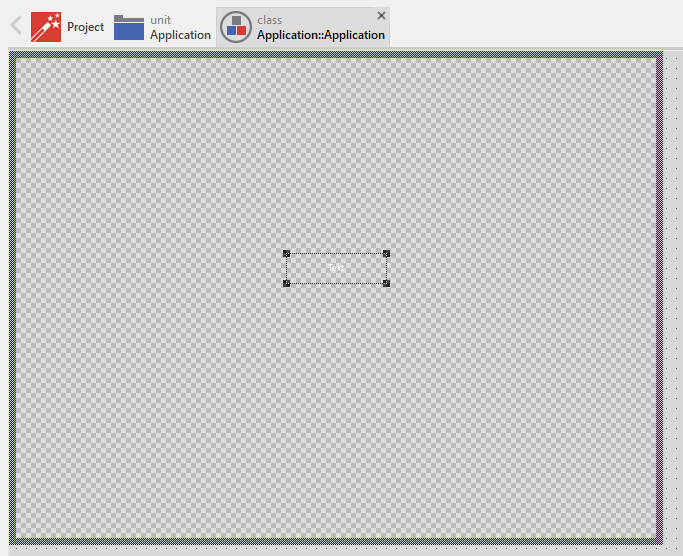
\includegraphics{./../asciidoc/modules/ROOT/assets/images/helloworld/RootCanvasTextView.png}
\caption{Root canvas with inserted text view}
\end{figure}

So far so good, let's style our text a bit to make it more appealing:

\begin{itemize}
\item
  In the composer window, click on the newly inserted text view to
  select the element.
\item
  Now have a look at the
  \href{https://doc.embedded-wizard.de/inspector-window}{inspector
  window} right to the main composer window: in the upper \emph{member
  area} you should see the element named \emph{Text} selected. Also note
  the attributes and properties area below that shows all properties of
  the currently selected text view.
\item
  Inside the attributes and properties area, we can adapt the newly
  inserted text view to our needs:

  \begin{itemize}
  \item
    Using the dropdown list, alter the \emph{Font} property of the text
    element to the value \emph{Resources::FontExtraLarge}.
  \item
    Using the dropdown element, alter the \emph{Color} property of the
    text element to the value \emph{\#000000FF} (black, opaque).
  \item
    In order to change the display text, alter the \emph{String}
    property of the text element to the value \emph{"Hello, world!"}.
  \item
    Since we do have text overflow in the element now, alter the
    \emph{AutoSize} property of the text element to the value
    \emph{true}.
  \end{itemize}
\end{itemize}

\begin{figure}
\centering
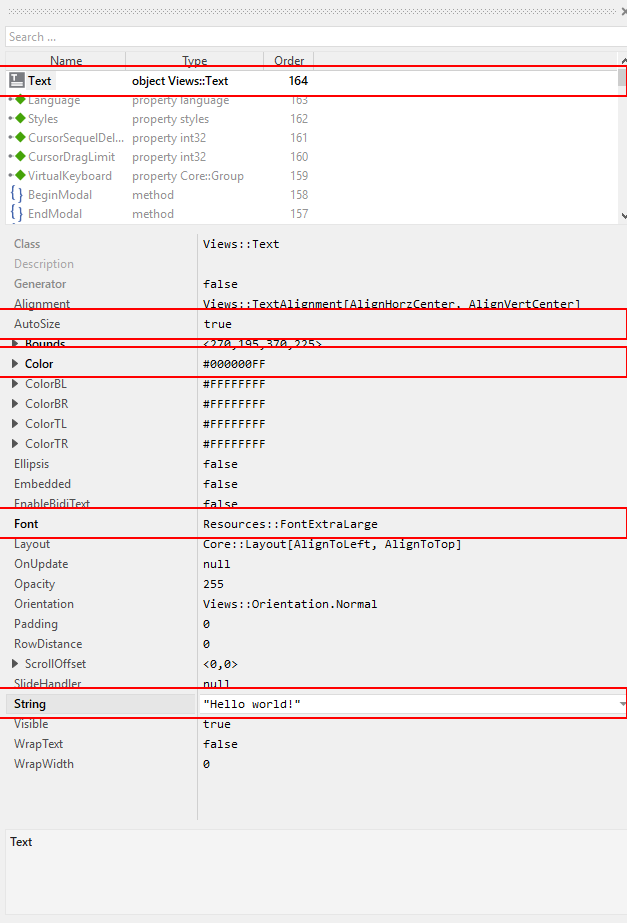
\includegraphics{./../asciidoc/modules/ROOT/assets/images/helloworld/PropertiesWindow.png}
\caption{Properties area with text view selected}
\end{figure}

That's it, we do have our message on the screen now!

\begin{quote}
\textbf{Important}

When typing in the \emph{Hello, world!} text, make sure that the string
you typed in is surrounded by double quotes, otherwise an error message
will come up.
\end{quote}

\hypertarget{_running_the_application}{%
\subsection{Running the application}\label{_running_the_application}}

Our \emph{Hello world} application is now ready to run!

There are several ways to launch the app:

\begin{itemize}
\item
  From the main menu, select the menu item \textsc{Build > Start prototyper
  with application class}, or
\item
  use the keystroke combination {[}Ctrl+F5{]}, or
\item
  click on the application launch icon
  
\includegraphics{./../asciidoc/modules/ROOT/assets/images/icons/LaunchApplicationIcon.png}
  in the second row of the toolbar.
\end{itemize}

Congratulations, you successfully assembled your first application!

Let's move on to the next \href{:FirstComponent.xml}{chapter}, there's
much more to explore here!

\chapter{Adding your first GUI component}

\rhead[]{Adding your first GUI component}

In the \href{:HelloWorld.xml}{last chapter}, we successfully built the
\emph{Hello world} application. In order to show the text, we placed a
text view element directly on the root canvas. While this is a valid
approach, it is highly recommended to build reusable components and use
these components when assembling your application. This approach has two
main benefits:

\begin{description}
\item[Testing]
Using the built-in protoyper, you can test the components in isolation.
There is a much higher chance the application works as expected once you
assemble it from already tested (sub-)components.
\item[Reusability]
When using components, it's much easier to follow the DRY principle
(\textbf{d}on't \textbf{r}epeat \textbf{y}ourself). You only write a
component once and may use it in several places.
\end{description}

So let's start and build our first GUI component: it's a simple
graphical unit with a border, a header text, a push button, and a
background. Once the button is pressed, some action will occur.

\hypertarget{_adding_the_empty_component_itself}{%
\section{Adding the empty component
itself}\label{_adding_the_empty_component_itself}}

\begin{itemize}
\item
  We want to place the component in the \emph{Application} unit, so
  click on the tab labelled \emph{Application}. If this tab is not
  present yet, click on the
  
\includegraphics{./../asciidoc/modules/ROOT/assets/images/icons/EmbeddedWizardIcon.png}
  \emph{Project} tab and double click on the \emph{Application} unit to
  invoke the tab. Inside the composer window, you will now see the
  \emph{Application} root component, the only component currently
  present.
\item
  Press {[}Alt+1{]} to put the focus on the
  \href{https://doc.embedded-wizard.de/gallery-templates-window}{gallery
  templates window}, left to the main composer window. Alternatively,
  you may mouse click at the tab \emph{Templates} at the very top of the
  window, to the left.
\item
  Press {[}C{]} twice: the first key press opens the
  \emph{\textbf{C}hora} folder, the second key press will then open the
  invoke folder \emph{\textbf{C}omponent templates}, that's what we
  need. Alternatively, you may mouse click on the header titled
  \emph{Component templates} inside the main area of the templates
  window. This will also open the folder and show all available GUI
  templates.
\item
  Identify the item 
\includegraphics{./../asciidoc/modules/ROOT/assets/images/icons/ComponentIcon.png}
  \emph{Component}, representing an empty GUI component. Click on the
  element, drag it into the main area and place it underneath the
  existing \emph{Application} root component.
\item
  We want to use the new component to ring a bell, so we give it a
  dedicated name: with the component still selected, press {[}F2{]}
  to rename the component. In the
  \href{https://doc.embedded-wizard.de/inspector-window}{inspector
  window}, type in \emph{BellComponent} and press {[}Enter{]} once
  you are done.
\end{itemize}

\begin{figure}
\centering
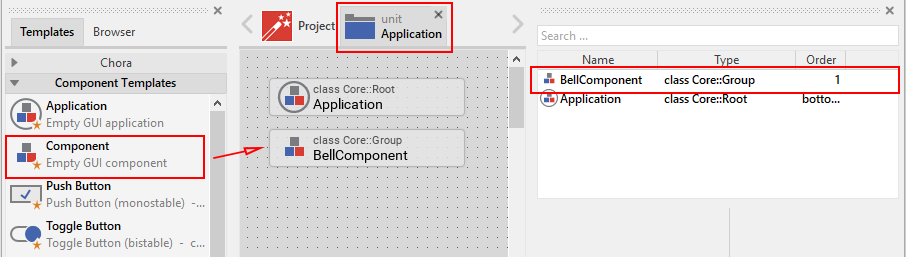
\includegraphics[keepaspectratio,width=5.5cm]{./../asciidoc/modules/ROOT/assets/images/firstcomponent/InsertingComponent.png}
\caption{Inserting an empty GUI component}
\end{figure}

Now, we have to open the empty component we just inserted:

\begin{itemize}
\item
  Double click on the newly inserted icon
  
\includegraphics{./../asciidoc/modules/ROOT/assets/images/icons/BellComponentIcon.png},
  representing the \emph{bell} component.
\item
  Inside the composer window, another tab appears which shows the
  contents of the component class which is now opened:
\end{itemize}

\begin{figure}
\centering
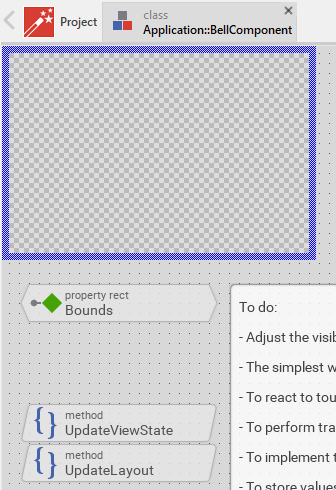
\includegraphics{./../asciidoc/modules/ROOT/assets/images/firstcomponent/EmptyComponent.png}
\caption{Empty GUI component}
\end{figure}

\hypertarget{_filling_the_component}{%
\section{Filling the component}\label{_filling_the_component}}

Next, we have to fill the empty component:

\begin{itemize}
\item
  First, we do some cleanup: With the {[}Shift{]} key pressed, click
  on the two methods \emph{UpdateViewState} and \emph{UpdateLayout} to
  select both methods. Press the {[}Delete{]} key to delete those
  methods, we don't need them for now.
\item
  Also, click on the note element that contains a lot of text. Press the
  {[}Delete{]} key to delete this element, too.
\item
  Our component should have a size of 200 × 150 px, so we have to adjust
  this: click on the property \emph{Bounds} (adorned by a green diamond)
  to select the element. Now, in the in the upper \emph{member area} of
  the inspector window right to the main composer window you should see
  the element named \emph{Bounds} selected. Also note the attributes and
  properties area below that shows all properties of the currently
  selected \emph{Bounds} property.
\item
  Inside the attributes and properties area, we can adapt the default
  bounds values to our needs:

  \begin{itemize}
  \item
    Click on the black triangle left to the \emph{Default} element.
    Multiple lines will show up which hold the values for the origin
    (\emph{x}, \emph{y}) and the size of the element
    (\emph{\textbf{w}idth}, \_\textbf{h}eight).
  \item
    Alter the \emph{w} instance property of the component to the value
    \emph{200} to set the default width of the component to 200~px.
  \item
    Alter the \emph{h} instance property of the component to the value
    \emph{150} to set the default height of the component to 150~px.
  \item
    In order to adapt the size of the component on the screen, click on
    the \emph{Reload} icon
    
\includegraphics{./../asciidoc/modules/ROOT/assets/images/icons/ReloadIcon.png}
    in the second row of the toolbar or press {[}F7{]} to reload the
    class. The blue border of the element will shrink to the new size
    then.
  \end{itemize}
\end{itemize}

\begin{figure}
\centering
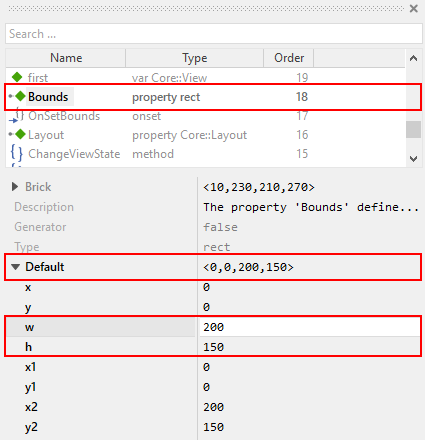
\includegraphics{./../asciidoc/modules/ROOT/assets/images/firstcomponent/ComponentBounds.png}
\caption{Setting the default component size}
\end{figure}

In a further step, we put all the elements onto the element's canvas:

\begin{itemize}
\item
  With the gallery templates window left to the main composer window
  focused ({[}Alt+1{]}), either click on the folder header
  \emph{Views} or press key {[}v{]}, this will open and show all
  items inside the \emph{\textbf{V}iew} folder.
\item
  Click on the item
  
\includegraphics{./../asciidoc/modules/ROOT/assets/images/icons/FilledRectangleIcon.png}
  \emph{Filled Rectangle}, and drag an instance over to the component's
  canvas. Place the element in the upper left corner of the canvas.
\item
  Press {[}F2{]} to rename the component. In the inspector window,
  type in \emph{Background} and press {[}Enter{]} once you are done.
\item
  Adapt the size of the background rectangle to 200 × 150 px. You may do
  so by either resizing the element with the mouse or by adjusting the
  property \emph{Bounds} in the in the lower \emph{attributes and
  properties area} of the inspector window (as described above when
  setting the default bounds for the component).
\item
  If needed, adjust the color of the background to the value
  \_\#FFFFFFFF (white, opaque).
\end{itemize}

Now we put a border around the component:

\begin{itemize}
\item
  In the gallery templates window, click on the item
  
\includegraphics{./../asciidoc/modules/ROOT/assets/images/icons/BorderIcon.png}
  \emph{Border} and drag an instance over to the component's canvas.
  Place the element in the upper left corner of the canvas.
\item
  Adapt the size of the border to 200 × 150 px. again, this may be done
  by either resizing the element with the mouse or by adjusting the
  property \emph{Bounds} of the component in the lower area of the
  inspector window.
\item
  Adjust the color of the border to the value \emph{\#000000FF} (black,
  opaque) and set the property \emph{Width} of the border to 1~px.
\item
  You now should see a black border around your component.
\end{itemize}

Next we add a header text to the component:

\begin{itemize}
\item
  In the \emph{gallery templates} window, click on the item
  
\includegraphics[scale=0.75]{./../asciidoc/modules/ROOT/assets/images/icons/TextViewIcon.png}
  \emph{Text} and drag an instance over to the component's canvas. Place
  the element centered in the upper area of the component.
\item
  Using {[}F2{]} key, rename the name to \emph{HeadingBell}.
\item
  Inside the attributes and properties area, adapt the newly inserted
  heading text to your needs:

  \begin{itemize}
  \item
    Using the dropdown list, alter the \emph{Font} property of the text
    element to the value \emph{Resources::FontExtraLarge}.
  \item
    Using the dropdown element, alter the \emph{Color} property of the
    text element to the value \emph{\#000000FF} (black, opaque).
  \item
    In order to change the display text, alter the \emph{String}
    property of the text element to the value \emph{"Bell"}.
  \item
    Since we do have text overflow in the element now, alter the
    \emph{AutoSize} property of the text element to the value
    \emph{true}.
  \end{itemize}
\end{itemize}

Eventually, we add the core element, a push button that will be used to
ring the bell:

\begin{itemize}
\item
  In the gallery templates window to the left, either click on the
  folder header \emph{\textbf{W}idgets} or press key {[}W{]}, this
  will open and show all items inside the \emph{\textbf{w}idgets}
  folder.
\item
  Click on the \emph{Push Button}, widget and drag an instance over to
  the component's canvas. Place the element in the lower area of the
  canvas.
\item
  Press {[}F2{]} to rename the component. In the inspector window,
  type in \emph{PushButtonBell} and press {[}Enter{]} once you are
  done.
\item
  Now customize the appearance of the push button. You may do so by
  setting the property \emph{Appearance} in the inspector window to
  \emph{WidgetSet::PushButtonSmall} and by setting the property
  \emph{Label} to \emph{Ring}.
\item
  You should now see a push button labelled \emph{Ring} in the lower
  area of the canvas.
\item
  In the search field at the very top of the inspector window, type in
  \emph{Focus} to look up the property \emph{Focus} of your component.
  By writing the string \emph{null} into the value input field, set the
  \emph{Default} value of this property explicitly to \emph{null}. An
  icon
  
\includegraphics{./../asciidoc/modules/ROOT/assets/images/icons/FocusPropertyIcon.png}
  \emph{Focus} will appear at the top left corner of the composer
  window, representing the overridden property. Move this icon to the
  bottom.
\end{itemize}

\begin{quote}
\textbf{Note}

By setting the \emph{Focus} to null, we prevent our component from
obtaining the focus. Obtaining the focus changes the component's
appearance, which is undesired in our case.
\end{quote}

We are finished now with adding elements to our component, and the
component should pretty much like shown in
\protect\hyperlink{fig:BellComponent}{figure\_title} below:

\begin{figure}
\centering
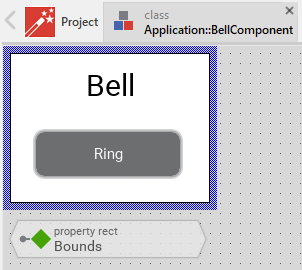
\includegraphics{./../asciidoc/modules/ROOT/assets/images/firstcomponent/BellComponentFinal.png}
\caption{Final look of bell component}
\end{figure}

\hypertarget{_defining_a_button_action_performed_on_click}{%
\section{Defining a button action performed on
click}\label{_defining_a_button_action_performed_on_click}}

So far, we successfully added elements the \emph{Bell} component. the
only interactive element is the push button, so let's bring life to this
component! To do so, we have to add some logic to the component, more
specifically some signal handler logic. Embedded Wizard heavily relies
on so called
\href{https://doc.embedded-wizard.de/slot-method-member}{slot methods}
when implementing communication between two objects. Slot methods show
the following characteristics:

\begin{description}
\item[Code based implementation]
Every slot method has a method body containing the logic that will be
performed once the slot method was called. The programming language used
when authoring code inside the method's body is \emph{Chora}:, a
relatively unknown, platform independent language which syntax closely
resembles C.
\item[Signal based communication between objects]
In order to invoke a slot method, a signal has to be send to the method.
Once the slot method receives the signal the code in the body of the
slot method is executed. Since a slot method does not take parameters,
signal-based process communication can happen between all kinds of
objects, the sender does not have to know about the identity of the
receiver object. However, the identity of the sender is passed onto the
slot method in the hidden parameter \emph{sender} which can be used
inside the body of the slot method.
\item[Inheritance]
Slot methods are members of class objects. If a class is derived from
another class, it inherits all slot methods from this class. As any
inherited members, these slot methods can be overridden if needed. You
also may call the inherited version ot the slot method by making use of
the pseudo method \emph{super()}.
\end{description}

So let's start and build our first slot method to bring life to our push
button:

\begin{itemize}
\item
  In the gallery templates window to the left, either click on the
  folder header \emph{\textbf{C}hora} or press key {[}w{]} twice,
  this will open the folder and will present the list of all language
  elements available in the programming language \emph{\textbf{C}hora}.
\item
  To keep our component organized, it's a good idea to place a note
  group on the canvas first:

  \begin{itemize}
  \item
    Click on the element
    
\includegraphics{./../asciidoc/modules/ROOT/assets/images/icons/AnnotationGroupIcon.png}
    \emph{Annotation Group}, and drag an instance over to the
    component's canvas. Place the element right beneath the component's
    canvas.
  \item
    By default, the heading of the note is \emph{This is an annotation}.
    Change the heading of the note area by changing the property
    \emph{Caption} in the inspector window to \emph{Slot method(s)}.
  \end{itemize}
\item
  By now we are ready to insert our slot method: Click on the element
  
\includegraphics{./../asciidoc/modules/ROOT/assets/images/icons/SlotMethodIcon.png}
  \emph{Slot Method}, and drag an instance over to the component's
  canvas. Place the element inside the note rectangle you inserted and
  adapted in the previous two steps.
\item
  Press {[}F2{]} to rename the slot method. In the inspector window,
  type in \emph{RingTheBellSlot} and press {[}Enter{]} once you are
  done.
\item
  Finally, we have to fill the body of the slot method with some code.
  To do so, double click on the icon
  
\includegraphics{./../asciidoc/modules/ROOT/assets/images/icons/RingTheBellSlotIcon.png}
  representing the slot method \emph{RingTheBellSlot}. In the
  \href{https://doc.embedded-wizard.de/code-editor-window}{Code editor},
  you will now see one single line of Chora code:
\end{itemize}

\begin{verbatim}
sender; /* the method is called from the sender object */
\end{verbatim}

For now, change this code line to:

\begin{verbatim}
trace "Sorry, the GUI cannot ring the bell!";
\end{verbatim}

The \href{https://doc.embedded-wizard.de/trace-statemen}{trace} is a
debugging statement that prints diagnostic output to the
\href{https://doc.embedded-wizard.de/log-window}{log window} located in
the lower left area of the screen.

We now finished with our slot method now, as soon as a signal will be
sent to the method, it will print it's output to the log window.
However, we haven't connected our slot method to our push button yet, so
let's move on and connect the sender (=~push button) with the slot slot
method in order to get the push button working!

\begin{itemize}
\item
  To do so, we have to select the push button first. Select it by either
  clicking on the button object in the composer area or by clicking on
  the element titled \emph{PushButtonBell}, listed in the upper
  \emph{member area} of the inspector window to the right.
\item
  With the push button selected, search for the property
  \emph{OnActivate} in the lower area of the inspector window. The
  property \emph{OnActivate} refers to a slot method, so as value type
  in \emph{RingTheBellSlot}. If you want to save typing, click on the
  small downwards triangle at the right hand side of the value field
  select the slot method \emph{PushButtonSlot} from the long list
  offered inside the dropdown area.
\end{itemize}

You are done with your first component, the layout should look like
shown in \protect\hyperlink{fig:BellComponentWithSlot}{figure\_title}
below:

\begin{figure}
\centering
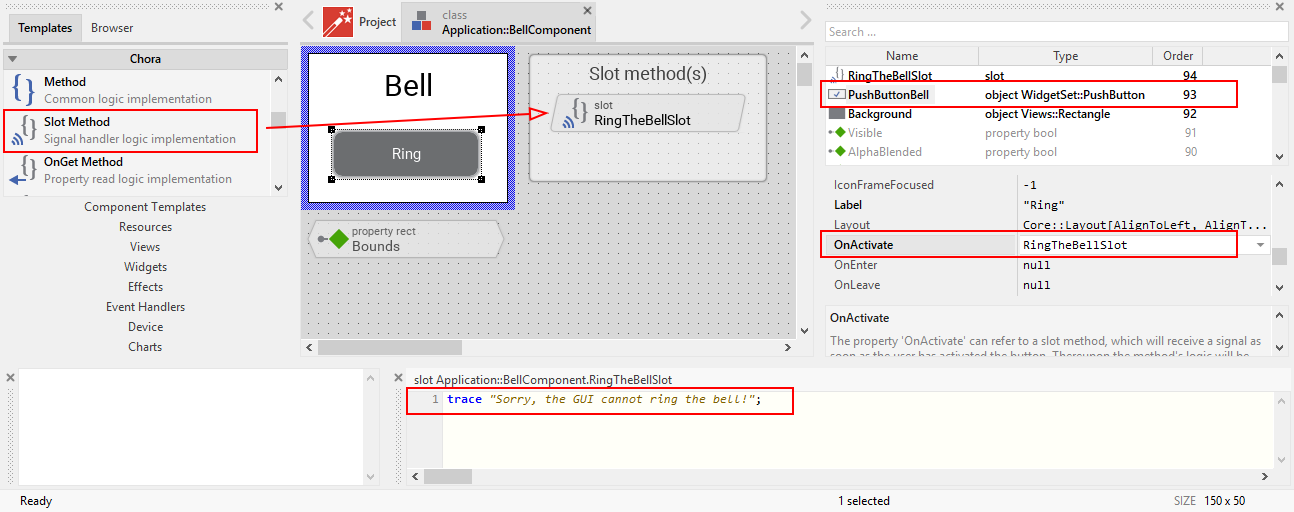
\includegraphics{./../asciidoc/modules/ROOT/assets/images/firstcomponent/BellComponentSlot.png}
\caption{Bell component with slot method defined}
\end{figure}

\hypertarget{_test_the_component_in_isolation}{%
\section{Test the component in
isolation}\label{_test_the_component_in_isolation}}

Let's go and test our first component! There are several ways to do so:

\begin{itemize}
\item
  From the main menu, select the menu item \textsc{Build > Start prototyper}, or
\item
  use the keystroke {[}F5{]}, or
\item
  click on the launch icon
  
\includegraphics{./../asciidoc/modules/ROOT/assets/images/icons/LaunchIcon.png}
  in the second row of the toolbar.
\end{itemize}

A prototyper window will appear which shows your component and simulate
its behaviour: Click on the push button, twice, and two debug messages
will appear in the log window:

\begin{figure}
\centering
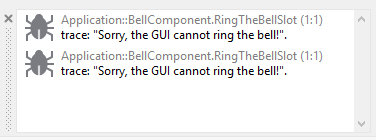
\includegraphics{./../asciidoc/modules/ROOT/assets/images/firstcomponent/DebugOutput.png}
\caption{Debugging output inside the log window}
\end{figure}

\begin{quote}
\textbf{Note}

When we launched the test above, the prototyper acted on a component
level, allowing us to test the component in isolation. We do also have
the opportunity to launch / prototype the whole application, use
{[}Ctrl+F5{]} to do so. Have a look at
\protect\hyperlink{tab:ProtoyperStart}{table\_title} which summarizes
the two different prototyping methods.
\end{quote}

\begin{longtable}[]{@{}lll@{}}
\caption{Starting the prototyper in different ways}\tabularnewline
\toprule
\begin{minipage}[b]{0.30\columnwidth}\raggedright
\strut
\end{minipage} & \begin{minipage}[b]{0.30\columnwidth}\raggedright
Prototyping of component\strut
\end{minipage} & \begin{minipage}[b]{0.30\columnwidth}\raggedright
Prototyping of application\strut
\end{minipage}\tabularnewline
\midrule
\endfirsthead
\toprule
\begin{minipage}[b]{0.30\columnwidth}\raggedright
\strut
\end{minipage} & \begin{minipage}[b]{0.30\columnwidth}\raggedright
Prototyping of component\strut
\end{minipage} & \begin{minipage}[b]{0.30\columnwidth}\raggedright
Prototyping of application\strut
\end{minipage}\tabularnewline
\midrule
\endhead
\begin{minipage}[t]{0.30\columnwidth}\raggedright
\textbf{Menu}\strut
\end{minipage} & \begin{minipage}[t]{0.30\columnwidth}\raggedright
Build > Start prototyper\strut
\end{minipage} & \begin{minipage}[t]{0.30\columnwidth}\raggedright
Build > Start prototyper with application class\strut
\end{minipage}\tabularnewline
\begin{minipage}[t]{0.30\columnwidth}\raggedright
\textbf{Keyboard shortcut}\strut
\end{minipage} & \begin{minipage}[t]{0.30\columnwidth}\raggedright
{[}F5{]}\strut
\end{minipage} & \begin{minipage}[t]{0.30\columnwidth}\raggedright
{[}Ctrl+F5{]}\strut
\end{minipage}\tabularnewline
\begin{minipage}[t]{0.30\columnwidth}\raggedright
\textbf{Toolbar icon}\strut
\end{minipage} & \begin{minipage}[t]{0.30\columnwidth}\raggedright

\includegraphics{./../asciidoc/modules/ROOT/assets/images/icons/LaunchIcon.png}\strut
\end{minipage} & \begin{minipage}[t]{0.30\columnwidth}\raggedright

\includegraphics{./../asciidoc/modules/ROOT/assets/images/icons/LaunchApplicationIcon.png}\strut
\end{minipage}\tabularnewline
\bottomrule
\end{longtable}

\hypertarget{_add_the_component_to_the_applications_root_component}{%
\section{Add the component to the application's root
component}\label{_add_the_component_to_the_applications_root_component}}

Having first component up and ready is pretty cool, isn't it? Let's move
on and integrate the component into the root component, that's what the
component is made for!

\begin{itemize}
\item
  Since want to place the component in the \emph{Application} unit,
  click on the tab labelled \emph{Application}. If this tab is not
  present yet, click on the
  
\includegraphics{./../asciidoc/modules/ROOT/assets/images/icons/EmbeddedWizardIcon.png}
  \emph{Project} tab and double click on the \emph{Application} unit to
  invoke the tab. Inside the composer window, you should now see the
  \emph{Application} root component and the \emph{Bell component},
  developed by you.
\item
  Rename the root application class to \emph{TutorialApplication} using
  the {[}F2{]} key.
\item
  Double click on the root application class that you just renamed. The
  root application class will be opened, showing the \emph{Hello world!}
  text we added in the last chapter.
\item
  Using the inspector window, change the \emph{Hello world!} text to
  \emph{Tutorial application}.
\item
  Using the \emph{Bounds} property, change the size of the root canvas
  to 480 × 320 px. If you don't know how to do that, have a look at how
  we changed the size of the \emph{bell} component above.
\item
  Add a background with the same dimensions of 480 × 320 px to the root
  canvas. If you don't know how to do that, have a look at how we added
  a background to the bell component above. Change the color of the
  background to Gainsborough (\emph{\#DCDCDCFF}).
\end{itemize}

\begin{quote}
\textbf{Important}

When adding the background onto the canvas, it will be placed in the
foreground and will hide your header text. In order to fix that, you
have to restack the elements on the canvas.

\begin{itemize}
\item
  Right click on the \emph{Background} element in the inspector window
  to show its context menu.
\end{itemize}

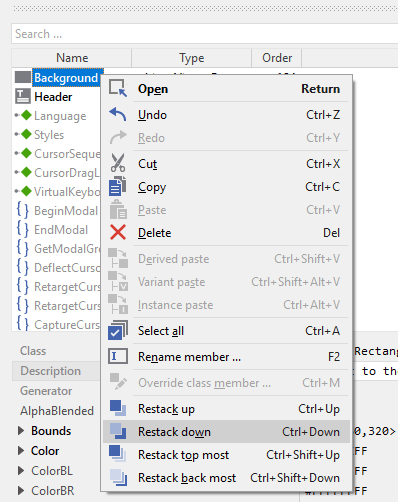
\includegraphics{./../asciidoc/modules/ROOT/assets/images/firstcomponent/RestackElements.png}

\begin{itemize}
\item
  From the context menu, select the menu item \emph{Restack down}.
\end{itemize}

\begin{quote}
\textbf{Tip}

When you want to restack an element several levels up or down, select
the element and then make use of the shortcuts {[}Ctrl+Up{]} or
{[}Ctrl+Down{]} respectively.
\end{quote}
\end{quote}

Now we are eventually ready to add our bell component:

\begin{itemize}
\item
  Press {[}Alt+2{]} to select the
  \href{https://doc.embedded-wizard.de/gallery-browser-window}{gallery
  browser window}, left to the main composer window. Alternatively, you
  may mouse click at the second tab \emph{Browser} at the very top of
  the window.
\item
  The browser's list of classes present is quite long, so we have to
  narrow down the displayed classes: in the search field immediately
  below the two tabs, type in \emph{Bell}. While typing have a look at
  the list and you will notice that the list is getting shorter and
  shorter. Once you typed in \emph{Bell}, the only class left is the
  component newly created by you.
\item
  Click on the
  
\includegraphics{./../asciidoc/modules/ROOT/assets/images/icons/ClassIcon.png}
  \emph{Application::BellComponent} class and drag an instance of the
  class over to the root canvas. Place the component below the header
  text.
\end{itemize}

Yeah! You successfully included your component into the main app!

\begin{figure}
\centering
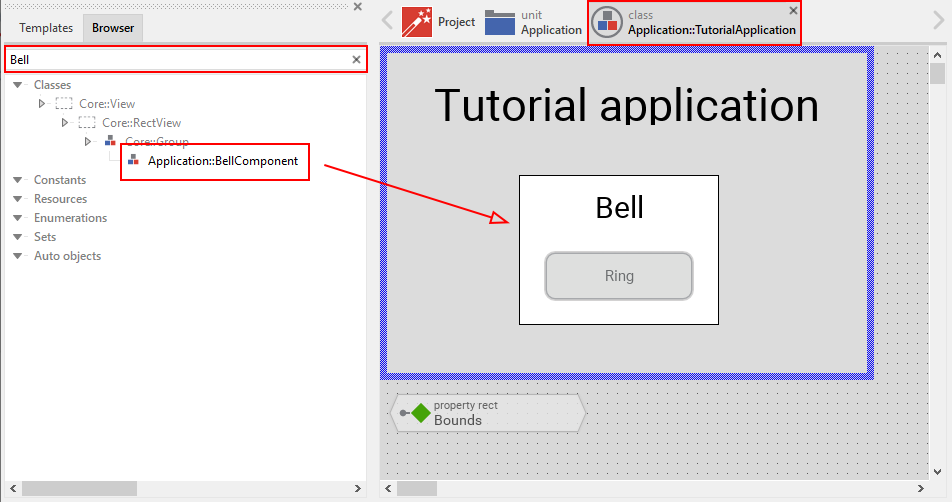
\includegraphics{./../asciidoc/modules/ROOT/assets/images/firstcomponent/TutorialApplication.png}
\caption{Tutorial application with bell component}
\end{figure}

Let's test it out:

\begin{itemize}
\item
  From the main menu, select the menu item \textsc{Build > Start prototyper}
  with application class{]}, or
\item
  use the keystroke combination {[}Ctrl+F5{]}, or
\item
  click on application launch icon
  
\includegraphics{./../asciidoc/modules/ROOT/assets/images/icons/LaunchApplicationIcon.png}
  in the second row of the toolbar.
\end{itemize}

The application will start up. You will notice that the screen size is
larger than the root element we put on it. Let's fix this:

\begin{itemize}
\item
  Click on the
  
\includegraphics{./../asciidoc/modules/ROOT/assets/images/icons/EmbeddedWizardIcon.png}
  \emph{Project} tab (the first tab from the left) and click on the
  \emph{Profile} item, located inside the note group \emph{Profile
  configuration}.
\item
  Using the inspector window, change the property \emph{ScreenSize} to
  \emph{\textless480,320\textgreater{}}.
\end{itemize}

\begin{figure}
\centering
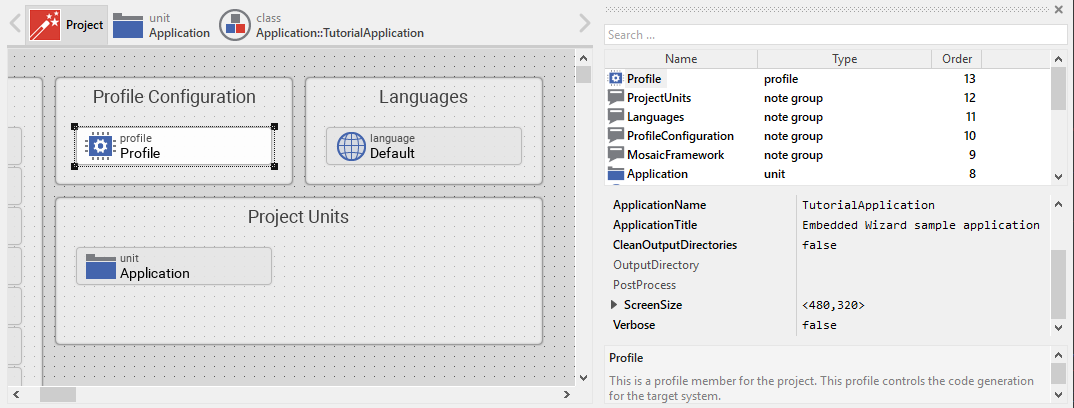
\includegraphics{./../asciidoc/modules/ROOT/assets/images/firstcomponent/AdaptingScreenSize.png}
\caption{Adapting the screen size}
\end{figure}

Hooray, it we have our first application up and running:

\begin{figure}
\centering
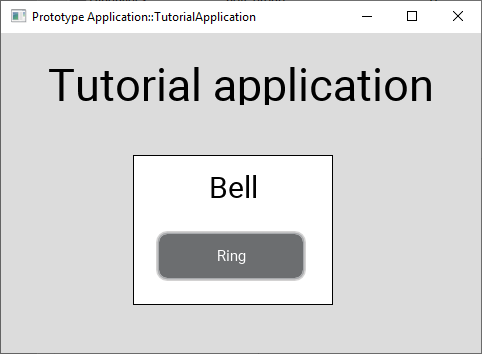
\includegraphics{./../asciidoc/modules/ROOT/assets/images/firstcomponent/TutorialApplicationRunning.png}
\caption{First application running}
\end{figure}

Let's move on to the \href{:ComponentReusability.xml}{next chapter},
there's still much more to explore!

\chapter{Making your component truly reusable}

\rhead[]{Making your component truly reusable}

In the \href{:FirstComponent.xml}{last chapter}, we successfully built
your first GUI component and put it on to the root canvas. As we saw,
this allows you to test your component in isolation, which is a great
benefit, especially when working on large scale projects. The second
motivation to use components is reusability. Let's think about this a
bit more: currently our bell component is tailored to ring a bell. This
somehow limits the reuse of the component. Of course you can put two or
more instances of the bell component on the root canvas, but it's
unlikely that anyone wants to have two ore more buttons on the screen
performing exactly the same action: ringing a bell. In a real world
application you often have several buttons, which all do perform
\emph{different} actions, however. With the components in its current
form, implementing this is not possible right now. So let's extend the
component and make it truly reusable in the next chapter!


\hypertarget{_extending_your_component_with_properties}{%
\section{Extending your component with
properties}\label{_extending_your_component_with_properties}}

Let's have a look at our component first:

\begin{itemize}
\item
  Open the the \emph{Application} unit by clicking on the tab labelled
  \emph{Application}. If this tab is not present yet, click on the
  
\includegraphics{./../asciidoc/modules/ROOT/assets/images/icons/EmbeddedWizardIcon.png}
  \emph{Project} tab and double click on the \emph{Application} unit to
  invoke the tab.
\item
  We want to refactor the \emph{BellComponent} in order to facilitate
  reuse of the component. This should be reflected in the name of the
  component, so go ahead and rename the component to
  \emph{PushButtonComponent} using the {[}F2{]} key.
\item
  Double click on the renamed \emph{PushButtonComponent} element. Its
  contents will be show in a new tab titled with the class name
  \emph{Application::PushButtonComponent}.
\end{itemize}

Let us reflect on the current design of the component a bit: currently
there are three items hard-coded, which severely limits the reusability
of this component:

\begin{itemize}
\item
  the text shown in the header text view (hard-coded value:
  \emph{Bell}),
\item
  the text of the label on the push button (hard-coded value:
  \emph{Ring}) and
\item
  the slot method attached to the property \emph{OnActivate} of the push
  button (hard-coded value: \emph{RingTheBellSlot}).
\end{itemize}

In order to allow reuse, we have to extend the component so that the
three items listed above can be stored inside the component. That's what
\href{https://doc.embedded-wizard.de/property-member}{properties} are
made for. If you do have a Java or C\# background, you already should be
familiar with the concept of properties:

\begin{itemize}
\item
  Properties are a kind of variable where data of an arbitrary Chora
  \href{https://doc.embedded-wizard.de/data-types}{data type} can be
  stored (e.g. string, int, slot, \ldots​). For each property, you have
  to specify the data type it can held (including its default value).
\item
  A property represents a more sophisticated variable in that sense that
  a property does have \emph{OnSet} and \emph{OnGet} methods that are
  used to get and set the value of the property. Normally, these methods
  contain boilerplate code that set or gets the internal memory of the
  property. You are encouraged to add your custom code to these
  method(s) to tailor them to your needs. We will do some shortly, so
  hold on!
\item
  You are allowed to attach slot methods as observer to any property we
  implement. As soon as the value of the property changes, the slot
  method (=~observer) gets notified about the change. This is a core
  feature of Chora that allows the development of applications following
  the
  \href{https://en.wikipedia.org/wiki/Model\%E2\%80\%93view\%E2\%80\%93controller}{MVC}
  pattern. We may talk about this later on.
\item
  Properties cannot only store arbitrary data type, they can also store
  references to any data type. Properties that store references are so
  called
  \href{https://doc.embedded-wizard.de/implementing-component-interface\#4}{outlet
  properties}. This is an advanced concept, we may talk about that later
  on.
\end{itemize}

That's the theory behind property in short, let's start and put theory
into practice:

First we have to make a few adjustments to our components in order to
reflect the refactoring of the component:

\begin{itemize}
\item
  In the \emph{PushButtonComponent} tab, rename the existing push button
  \emph{PushButtonBell} to \emph{PushButton} . Change the value of the
  property \emph{Label} of this component from \emph{"Ring"} to
  \emph{"Action"}.
\item
  Afterwards, rename the header text element \emph{HeadingBell} to
  \emph{Header} and change the value of the property \emph{Label} of
  this component from \emph{"Ring"} to \emph{"Action"}.
\item
  Delete both the existing slot method \emph{RingTheBellSlot} and the
  corresponding note group \emph{Slot method(s)} using the {[}Del{]}
  key. When using the refactored component, slot methods will be added
  on the root application level and not at the component level any more.
\item
  Remove the current value \emph{RingTheBellSLot} from the the property
  \emph{OnActivate} of the PushButton, otherwise you will run in trouble
  later on. To do so, select the \emph{PushButton} component and right
  click on its property \emph{OnActivate}. From the context menu select
  the menu item \emph{Restore default value} ({[}Ctrl+R{]}), and the
  current entry will be replace with the default \emph{null} value.
\end{itemize}

Let's get our feet wet and add some properties to our component:

\begin{itemize}
\item
  From the gallery templates window ({[}Alt+1{]}) with folder
  \emph{\textbf{C}hora} opened (key {[}C{]}), drag an instance of
  the
  
\includegraphics{./../asciidoc/modules/ROOT/assets/images/icons/AnnotationGroupIcon.png}
  \emph{Annotation Group} to the component's canvas. Place the element
  right beneath the component's canvas and rename the property
  \emph{Caption} of the element to \emph{Properties} using the inspector
  window.
\item
  Now we are ready to insert our properties: Click on the element
  
\includegraphics{./../asciidoc/modules/ROOT/assets/images/icons/PropertyIcon.png}
  \emph{Property}, and drag an instance over to the component's canvas.
  Place the element inside the note rectangle you inserted and adapted
  in the previous step.
\end{itemize}

As you can see, a property named \emph{Property} was inserted, together
with its \emph{OnSet} and \emph{OnGet} methods:

\begin{figure}
\centering
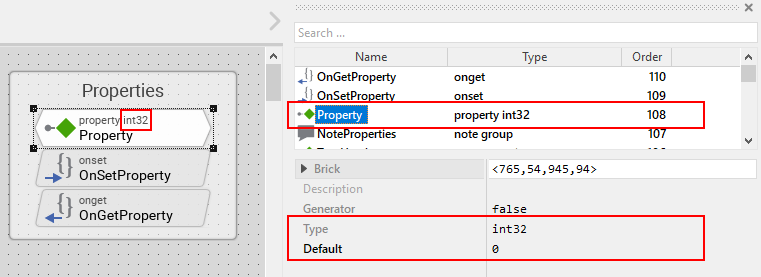
\includegraphics{./../asciidoc/modules/ROOT/assets/images/reusablecomponent/NewProperty.png}
\caption{Inserting our first property}
\end{figure}

Let's move on and adapt the property to our needs:

\begin{itemize}
\item
  The property should be used to store the text of the header element of
  our component, therefore we rename the property to \emph{TextHeader}
  using the {[}F2{]}. Please note that the names of the \emph{OnSet}
  and \emph{OnGet} methods automatically change to
  \emph{OnSetTextHeader} and \emph{OnGetTextHeader} respectively.
\item
  Currently, the data type of the property is \emph{int32}, that's not
  what we want, instead we want to store a string value (=~the header
  text) inside the property. To be able to do so, we change the value of
  the property \emph{Type} to \emph{string} inside the inspector window.
\item
  The header text of our component should be \emph{Header} by default,
  so we change the value \emph{Default} to \emph{"Header"} inside the
  inspector window. Don't forget the surrounding double quotes here or
  you may run in trouble.
\end{itemize}

The property is now set up to store the header text value. Currently,
when setting the header text property, the change of the property value
is not reflected inside the component. To overcome this, we have to add
some code to the OnSet method which is called each time a new value is
assigned to the property.

\begin{itemize}
\item
  Double click on the method \emph{OnSetTextHeader} of the property. In
  the code editor window, you will now see some lines of boilerplate
  Chora code:
\end{itemize}

\begin{verbatim}
// The value doesn't change - nothing to do.
if ( pure Property == value )
  return;

// Remember the property's new value.
pure Property = value;

// TO DO:
//
// Now you can handle the alternation of the property.
\end{verbatim}

Replace the \emph{TO DO:} section at the bottom with two lines of custom
code:

\begin{verbatim}
// The value doesn't change - nothing to do.
if ( pure Property == value )
  return;

// Remember the property's new value.
pure Property = value;

// change the text of the header
Heading.String = value;
\end{verbatim}

Our new line of code assigns the property \emph{String} of the
\emph{Heading} element (\emph{Heading.String}) the new value the
property was set to, this is immediately reflected in the GUI. That's
all we have to do! Now, as soon as the property gets a new value
assigned, the header text changes, too.

The first property is ready to go, so add two more properties:

\begin{itemize}
\item
  From the gallery templates window drag another
  
\includegraphics{./../asciidoc/modules/ROOT/assets/images/icons/PropertyIcon.png}
  \emph{Property} to the component's canvas.
\item
  Rename the property to \emph{LabelButton} using the {[}F2{]} key.
\item
  Change the type of the property to \emph{string}, with a default value
  \emph{"Label"}.
\item
  In the body of the \emph{OnSetLabelButton} method, replace the
  \emph{TO DO:} section with the code line
  \texttt{PushButton.Label\ =\ value;}.
\end{itemize}

This way, any change of the property \emph{LabelButton} will immediately
change the label text of the button. So far so good. Now we have to take
care that not only the label and heading text can be set, but also the
action performed once the button is clicked:

\begin{itemize}
\item
  From the gallery templates window drag another
  
\includegraphics{./../asciidoc/modules/ROOT/assets/images/icons/PropertyIcon.png}
  \emph{Property} to the component's canvas.
\item
  Rename the property to \emph{ActionButton} using the {[}F2{]} key.
\item
  Change the type of the property to \emph{slot}, with a default value
  \emph{null}.
\item
  In the body of the \emph{OnSetActionButton} method, replace the
  \emph{TO DO:} section with the code line
  \texttt{PushButton.OnActivate\ =\ value;}.
\end{itemize}

The refactoring of our component is done, it should now look like this:

\begin{figure}
\centering
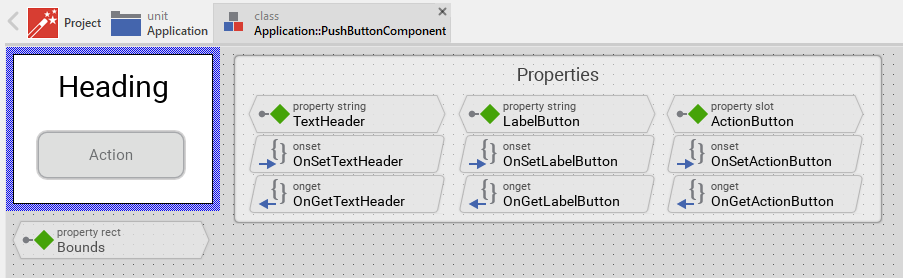
\includegraphics{./../asciidoc/modules/ROOT/assets/images/reusablecomponent/RefactoredComponent.png}
\caption{Refactored component}
\end{figure}

\hypertarget{_adapt_and_fix_the_main_application}{%
\section{Adapt and fix the main
application}\label{_adapt_and_fix_the_main_application}}

Now that refactoring our component is done, we have to make some changes
in the main application to make the application work again:

\begin{itemize}
\item
  Bring up the contents of the main application in the tab
  \emph{Application::TutorialApplication}.
\item
  The refactored pushbutton component now shows \emph{Header} as header
  text and \emph{Label} as button label. These are the default values of
  the properties we just introduced to the component. Let's customize
  the component's properties, that's why we introduced them in our
  component:
\item
  Using the inspector window, change the property of the push button
  component \emph{TextHeader} text to \emph{Bell}.
\item
  Using the inspector window, change the property \emph{LabelButton}
  text to \emph{Ring}.
\end{itemize}

The appearance of our component now again looks as wanted. When pressing
the button, nothing happens yet. Let's fix that, too:

\begin{itemize}
\item
  From the gallery templates window to the left, drag an element
  
\includegraphics{./../asciidoc/modules/ROOT/assets/images/icons/AnnotationGroupIcon.png}
  \emph{Annotation Group}, over to root canvas. Rename the group to
  \emph{Slot method(s)}.
\item
  Add a new slot method inside the note rectangle. Rename the slot
  method to \emph{RingTheBellSlot}.
\item
  Fill the body of the slot method with the code line
  \texttt{trace\ "Sorry,\ the\ GUI\ cannot\ ring\ the\ bell!";}.
\item
  Using the inspector window, change the property \emph{ActionButton} of
  the bell push button component to the newly created
  \emph{RingTheBellSlot}.
\end{itemize}

That's it! Test the main application in the prototyper
({[}Ctrl+F5{]}), and the main app should behave exactly as prior to
the refactoring.

\hypertarget{_adding_a_second_component_weather_forecast}{%
\section{Adding a second component (weather
forecast)}\label{_adding_a_second_component_weather_forecast}}

If you are asking yourself why we did the refactoring, things are
getting clear hopefully as soon as we insert a second instance of the
component. The GUI allows ringing the bell of your device already.
Imagine your device is able to present the weather forecast to you.
Maybe your device has a screen display for that purpose, or it has a
speaker to read out the forecast loud. Let's extend the GUI with a
second push button component for presenting the weather forecast to you:

\begin{itemize}
\item
  Press {[}Alt+2{]} to select the gallery browser window, left to
  the main composer window. Alternatively, you may mouse click at the
  second tab \emph{Browser} at the very top of the window.
\item
  In the search field immediately below the two tabs, type in
  \emph{Push} to shorten the class list.
\item
  Click on the
  
\includegraphics{./../asciidoc/modules/ROOT/assets/images/icons/ClassIcon.png}
  \emph{Application::PushButtonComponent} class and drag a second
  instance of the class over to the root canvas. Rearrange the two push
  button components so that both of them fit on the screen.
\end{itemize}

Yeah! You successfully included a second push button component into the
main app. Let's move on and customize the newly inserted component!

\begin{itemize}
\item
  If not already select, select the newly inserted component first:
\item
  Using the inspector window, change the property \emph{TextHeader} of
  the new push button component to the text string \emph{"Forecast"}.
\item
  Using the inspector window, change the property \emph{LabelButton} of
  the same component to \emph{"Show"}.
\item
  Add a new slot method inside the note rectangle titled \emph{Slot
  methods}. Rename the slot method to \emph{ForecastSlot}.
\item
  Fill the body of the slot method with the code line
  \texttt{trace\ "Sorry,\ but\ the\ GUI\ cannot\ tell\ the\ weather\ forecast";}.
\item
  Using the inspector window, change the property \emph{ActionButton} of
  the new push button component to the newly created
  \emph{ForecastSlot}.
\end{itemize}

The extended version of the application with two push button components
should now look like in
\protect\hyperlink{fig:ExtendedApplication}{figure\_title} below:

\begin{figure}
\centering
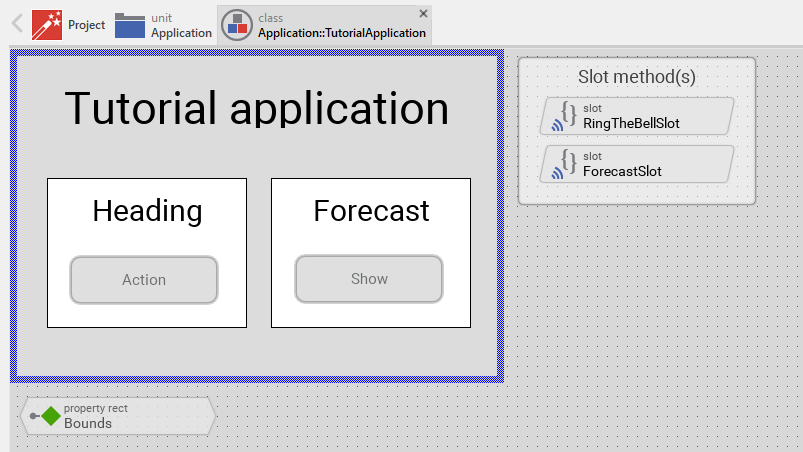
\includegraphics{./../asciidoc/modules/ROOT/assets/images/reusablecomponent/TutorialApplicationExtended.png}
\caption{Extended tutorial application}
\end{figure}

Go ahead and test your application! You should see different debugging
output depending on the button pressed.

This chapter has come to an end, time to recap: By adding three
properties to our component we managed to create a truly reusable
component. Creating reusable components comes has its price, however,
this will certainly pay off once your project grows over time.

Let's move on to the \href{:DeviceIntegrationBrowser.xml}{next chapter},
there's still much more to explore!

\chapter{Device integration: Hello world from our device}

\rhead[]{Device integration: Hello world from our device}

In the \href{:ComponentReusability.xml}{last chapter}, we made our
component truly reusable by adding properties to it. Afterwards we
completed our GUI which now contains two units, one for ringing a bell
and another for showing the weather forecast. Unfortunately, there's no
real function behind the push buttons of both units yet. We will address
this in the following chapter.

\hypertarget{_gui_builder_and_platform_packages}{%
\section{GUI builder and platform packages}\label{_gui_builder_and_platform_packages}}

Embedded Wizard is a GUI framework builder that allows you to build GUI
platform independent applications that can deployed on many different
target systems. This is achieved by using the programming language Chora
for all programming tasks related to the GUI. Other than that, Embedded
Wizards strictly refrains from any access to the underlying device to
ensure platform independence. However, when building embedded devices,
the main purpose of the GUI application is to enable and facilitate
interaction with the underlying hardware. So how does Embedded Wizard
integrate with those devices? That's where the concept of
\href{https://doc.embedded-wizard.de/platform-package}{platform
packages} comes into play. Embedded Wizard offers platform packages for
many different hardware platforms (STM, NXP, TI, Raspberry Pi, \ldots​).
A platform package consists of a code generator, a resource converter, a
graphics engine and a runtime environment for the specific platform. You
may think of the platform package as a link between the GUI and the
hardware. Applications implemented in the programming language Chora can
be run on any particular platform if a platform package exists for that
platform.

\hypertarget{_adapting_the_project_structure}{%
\section{Adapting the project
structure}\label{_adapting_the_project_structure}}

As explained above, there is a strict separation between the GUI
application and the device, represented by one or more platform
packages. Let's start and reflect that separation in our application
structure, too:

\begin{itemize}
\item
  Click on the
  
\includegraphics{./../asciidoc/modules/ROOT/assets/images/icons/EmbeddedWizardIcon.png}
  \emph{Project} tab (the first tab from the left).
\item
  Identify the note frame that holds the icon
  
\includegraphics{./../asciidoc/modules/ROOT/assets/images/icons/ApplicationUnitIcon.png}
  that represents the application unit. Rename the heading text of this
  frame from \emph{Project Units} to \emph{GUI project}. To do so,
  change the property \emph{Caption} of the note frame using the
  inspector window.
\item
  From the gallery templates window to the left, drag an element
  \includegraphics{./../asciidoc/modules/ROOT/assets/images/icons/AnnotationGroupIcon.png}
  \emph{Annotation Group} over to root canvas. Rename the group to
  \emph{Middleware}.
\item
  Drag an element
  \includegraphics{./../asciidoc/modules/ROOT/assets/images/icons/UnitIcon.png}
  \emph{Unit} over to root canvas, add the new unit inside the note
  rectangle you inserted in the previous step. Rename the unit to
  \emph{Device}.
\item
  Drag another
  \includegraphics{./../asciidoc/modules/ROOT/assets/images/icons/UnitIcon.png}
  \emph{Unit} into the same note rectangle \emph{Middleware}. Rename the
  unit to \emph{BrowserDevice}.
\item
  Drag a third
  \includegraphics{./../asciidoc/modules/ROOT/assets/images/icons/UnitIcon.png}
  \emph{Unit} into the note rectangle \emph{Middleware}. Rename the unit
  to \emph{TargetDevice}.
\end{itemize}

The structure of your project should now look as shown in
\protect\hyperlink{fig:ExtendedProjectLayout}{figure\_title} below:

\begin{figure}
\centering
\includegraphics{./../asciidoc/modules/ROOT/assets/images/deviceintegration/ProjectStructure.png}
\caption{Extended project layout}
\end{figure}

\hypertarget{_adding_a_interface_device_class}{%
\section{Adding a interface device
class}\label{_adding_a_interface_device_class}}

Let's add content to the newly inserted units! We start with adding a
device class interface first:

\begin{itemize}
\item
  Double click on the icon
  \includegraphics{./../asciidoc/modules/ROOT/assets/images/icons/DeviceUnitIcon.png},
  representing the \emph{Device} unit. This will open the unit in a new
  tab.
\item
  In the gallery templates window left to the main composer window
  ({[}Alt+1{]}), either click on the folder header
  \emph{\textbf{D}evice} or press key {[}D{]}, this will open the
  folder and will present all \emph{\textbf{d}evice} subitems.
\item
  Click on the item
  \includegraphics{./../asciidoc/modules/ROOT/assets/images/icons/DeviceInterfaceIcon.png}
  \emph{Device interface}, and drag an instance over to the component's
  canvas. Place the element in the upper left corner of the canvas.
\end{itemize}

By dragging over the \emph{device interface} to the canvas, two new
objects were inserted:

\begin{itemize}
\item
  the \emph{DeviceClass} element to the left, which represents the class
  where we will store device related class members like commands,
  properties and so on, and
\item
  the \emph{Device} autoobject element associated to the
  \emph{DeviceClass} element. This autoobject represents the globally
  available instance of the device class. This autoobject represents
  Embedded Wizard's implementation of the
  \href{https://en.wikipedia.org/wiki/Singleton_pattern}{singleton
  pattern} (if you are familiar with Java, you may think of the
  \emph{Device} class as a static class). Using the \emph{Device}
  autoobject, any GUI element has direct access to the device class and
  its members, which is very handy. We will use this autoobject soon.
\end{itemize}

Your screen should now look like illustrated in
\protect\hyperlink{fig:DeviceClassInterface}{figure\_title} below:

\begin{figure}
\centering
\includegraphics{./../asciidoc/modules/ROOT/assets/images/deviceintegration/DeviceClassInterface.png}
\caption{Device class interface}
\end{figure}

Let's go ahead and review and adapt the members of the newly inserted
device class interface:

\begin{itemize}
\item
  Double click on the icon
  \includegraphics{./../asciidoc/modules/ROOT/assets/images/icons/DeviceAutoObjectIcon.png},
  representing the \emph{Device} autoobject. This will open the
  \emph{Device} class in a new tab. You will see that the canvas was
  prepopulated with several class members already.
\item
  Identify the note group that holds the icon
  \includegraphics{./../asciidoc/modules/ROOT/assets/images/icons/CommandMethodIcon.png}
  representing the \emph{Command} method and rename the caption of this
  note group from \emph{Example of an interface to perform an operation
  in the device} to \emph{Command(s)}.
\item
  Rename icon
  \includegraphics{./../asciidoc/modules/ROOT/assets/images/icons/CommandMethodIcon.png}
  representing the \emph{Command} method to \emph{RingTheBellCommand}.
\item
  Double click on the renamed command. In the code editor window, you
  will see the method's signature, followed by many lines of template
  Chora code.
\item
  Have a look at the method signature of the \emph{RingTheBell} command.
\end{itemize}

Device commands are represented by regular methods. Like in all
programming languages, a method can take parameters and can have a
return value. Have a look at the signature of the
\emph{RingTheBellCommand} method shown at the top of the code editor:

\begin{verbatim}
 method int32 Device::DeviceClass.RingTheBellCommand( arg int32 aParameter1, arg bool aParameter2)
\end{verbatim}

As you can see the method currently takes an int32 value as first
argument and a boolean value as second argument. Also, the method
returns an int32 value. These settings are not what we want, our simple
\emph{RingTheBellCommand} method does not need any parameters and won't
return anything, so the return type should be \emph{void}. Let's go
ahead and adjust the method's signature to our needs:

\begin{itemize}
\item
  In the top title line of the code editor containing the method
  signature, you can see a small downwards triangle. Click on this
  triangle to show a frame where the method's return value and
  parameters are listed in separate lines.
\item
  Right click on the first method parameter \emph{arg int32 aParameter1}
  to invoke the context menu on this parameter. From this menu select
  the menu item \emph{Delete} to remove the first parameter.
\item
  Right click on the remaining method parameter \emph{arg bool
  aParameter2}. From the context menu shown, select \emph{Delete} to
  remove this parameter, too.
\item
  Right click on the first line that shows the method's name
  \emph{method int32 RingTheBellCommand}. From the context menu shown,
  select \emph{Edit} and change the return parameter from \emph{int32}
  to \emph{void}.
\end{itemize}

\begin{figure}
\centering
\includegraphics{./../asciidoc/modules/ROOT/assets/images/deviceintegration/DeleteMethodParameters.png}
\caption{Delete methods parameters}
\end{figure}

Once we adjusted the signature of the method, let us adjust the body of
the method, too. Remove all template code and put in one single line:

\begin{verbatim}
trace "The device class of the GUI is an interface only and cannot run any device commands! Please implement the command in a variant class!";
\end{verbatim}

As said, Embedded Wizard does not have access to the underlying device
and therefore cannot advise the device to say \emph{Hello} to us. We
have to implement this in a derived class, we will do so shortly.

Since we have set up a device and a command now, let's use it and wire
the push button action of the bell to that newly created command:

\begin{itemize}
\item
  Bring up the contents of the main application inside the tab
  \emph{Application::TutorialApplication}.
\item
  Double click on the icon
  \includegraphics{./../asciidoc/modules/ROOT/assets/images/icons/RingTheBellSlotIcon.png}
  representing the slot method \emph{RingTheBellSlot}. Inside the code
  editor, you will see the line
  \texttt{trace\ "Sorry,\ the\ GUI\ cannot\ ring\ the\ bell!";}.
\end{itemize}

Change this code to

\begin{verbatim}
Device::Device.RingTheBellCommand();
\end{verbatim}

\begin{quote}
\textbf{Note}

Embedded Wizard code editor ships with integrated code completion, which
is very handy and might prevent you from typos when authoring code
inside the code editor. To test it out, simply write \emph{Device::}
into the editor and should see a list of available completions to the
given \emph{Device} unit name you just typed in.
\end{quote}

That's how we call a method by code: specify the class name
(\emph{Device::DeviceClass}) first, then append the method name
(\emph{RingTheBellCommand}), prepended with a dot and terminated with
empty parentheses. Now run your code using the prototyper, and you
should see a trace message informing you that the GUI cannot run any
device commands. Obviously, we are not at the end, so read on!

\hypertarget{_adding_another_profile}{%
\section{Adding another profile}\label{_adding_another_profile}}

As already explained above, there is a strict separation between the GUI
application and the device, represented by one or more platform
packages. Two platform packages are included in the Embedded Wizard
installer and are available out of the box:

\begin{itemize}
\item
  the \emph{Tara.Win32.xxx} platform package. This is the default
  platform package that allows you to run the application on your
  Windows platform. You were using it already when you launched the
  prototyper to run your application or component (\emph{xxx} stand for
  one of the available color formats, either Index8 or RGBxxxxx).
\item
  the \emph{Tara.WebGL.RGBA8888} platform. This WebGL/Javascript
  platform package allows you to run the GUI in any WebGL enabled
  browser. That's especially handy for this tutorial since you don't
  need any hardware to follow the instruction given.
\end{itemize}

\begin{quote}
\textbf{Note}

Besides the Win32 and the WebGL packages there are many platform
packages available to target real hardware (STM, NXP, TI, Raspberry Pi,
\ldots​). For each of these platform packages, a separate installer
exists. You have to obtain and run this installer to make the associated
platform packages available inside Embedded Wizard.
\end{quote}

If we want to make use of more than one platform package inside our
project, we have to have an associated
\textbf{\href{https://doc.embedded-wizard.de/profile-member}{profile}}
on the Projects tab for each package you would like to use. So let's add
another profile that allows us to switch between the Win32 package and
the WebGL package. We then use the latter package to output \emph{Hello,
world!} on the browser device, more specifically on the web console of
the browser. The journey goes on \ldots​

\begin{itemize}
\item
  Click on the
  \includegraphics{./../asciidoc/modules/ROOT/assets/images/icons/EmbeddedWizardIcon.png}
  \emph{Project} tab (the first tab from the left).
\item
  Identify the note frame with the caption \emph{Profile configuration},
  it only contains the icon
  \includegraphics{./../asciidoc/modules/ROOT/assets/images/icons/DefaultProfileIcon.png}
  representing the default profile. Select this profile and have a look
  at the inspector window. You will realize that the attribute
  \emph{PlatformPackage} of the profile has the value
  \emph{Tara.Win32.RGBA8888} assigned. To reflect this, rename the
  profile from \emph{Profile} to \emph{Win32} using the {[}F2{]}
  key.
\item
  From the gallery templates window to the left, drag the element
  \includegraphics{./../asciidoc/modules/ROOT/assets/images/icons/ProfileIcon.png}
  \emph{Profile} inside the \emph{Chora} folder over to the canvas and
  place it underneath the existing profile \emph{Win32} . Rename the
  profile to \emph{Browser}. Resize the note frame and rearrange the
  elements on the canvas so that the layout looks nice again.
\item
  Our new profile should be associated with the WebGL platform package,
  so inside the inspector window, change the value of the attribute
  \emph{PlatformPackage} from \emph{Tara.Win32.RGBA8888} to
  \emph{Tara.WebGL.RGBA8888}.
\item
  Inside the inspector window, change the value of the attribute
  \emph{ScreenSize} to \emph{\textless480,320\textgreater{}}.
\item
  Also change the value of the attribute \emph{OutputDirectory} to
  \emph{../WebGL}. This defines the directory where all the code for our
  website will be stored once we build the project.
\item
  Optionally, you may fill the attributes \emph{ApplicationName} and
  \emph{ApplicationTitle} with the values \emph{TutorialApplication} or
  \emph{"Embedded Wizard sample application"}, respectively. For the
  last value, don't forget the surrounding double quotes here or you may
  run in trouble.
\end{itemize}

The \emph{Profile} section of your project should now look as shown in
\protect\hyperlink{fig:ProjectProfiles}{figure\_title} below:

\begin{figure}
\centering
\includegraphics{./../asciidoc/modules/ROOT/assets/images/deviceintegration/ProjectProfiles.png}
\caption{Project profiles and their attributes}
\end{figure}

\begin{quote}
\textbf{Tip}

Now that we have two profiles defined, we can switch between these two
profiles using the
\href{https://doc.embedded-wizard.de/menu-build\#9}{\emph{Profile}
dropdown list} located in the second row of the toolbar, placed right
beneath the icon
\includegraphics{./../asciidoc/modules/ROOT/assets/images/icons/BuildProfileIcon.png}
for building the selected profile and the icon
\includegraphics{./../asciidoc/modules/ROOT/assets/images/icons/BuildBatchIcon.png}
for building multiple profiles in batch mode:

\begin{figure}
\centering
\includegraphics{./../asciidoc/modules/ROOT/assets/images/deviceintegration/DropdownProfiles.png}
\caption{Dropdown list for switching between different profiles}
\end{figure}
\end{quote}

\hypertarget{_adding_a_browser_device_class_variant}{%
\section{Adding a browser device class
variant}\label{_adding_a_browser_device_class_variant}}

We already added an interface device class to our project. However, this
interface device class is not meant to run any command on the device.
The actual execution of the command on the device will happen inside a
\href{https://doc.embedded-wizard.de/class-variant-member}{class
variant}.
\href{https://doc.embedded-wizard.de/managing-project-variants}{Variants}
are an extremely powerful concept of Embedded wizard, in the example
below we use it to manage code execution on different platform packages.
Variants are useful in various other scenarios, you may use them to
manage variants of your application for different screen resolutions or
if you want to implement a different look and feel for one or more
application components. Let's go ahead and add and populate a class
variant for the use with browser devices:

\begin{itemize}
\item
  Click on the
  \includegraphics{./../asciidoc/modules/ROOT/assets/images/icons/EmbeddedWizardIcon.png}
  \emph{Project} tab (the first tab from the left).
\item
  Identify the note frame with the caption \emph{Middleware} which holds
  three device units, the \emph{Device} unit, the \emph{BrowserDevice}
  unit and the \emph{TargetDevice} unit.
\item
  Double click on the icon
  \includegraphics{./../asciidoc/modules/ROOT/assets/images/icons/BrowserDeviceUnitIcon.png},
  representing the \emph{BrowserDevice} unit. This will open the empty
  unit inside a new tab.
\item
  Press {[}Alt+2{]} to select the
  \href{https://doc.embedded-wizard.de/gallery-browser-window}{gallery
  browser window}, left to the main composer window. Alternatively, you
  may mouse click at the second tab \emph{Browser} at the very top of
  the window.
\item
  In the search field immediately below the two tabs, type in
  \emph{Device} to shorten the class list.
\item
  Right click on the
  \includegraphics{./../asciidoc/modules/ROOT/assets/images/icons/ClassIcon.png}
  \emph{Device::DeviceClass} class to invoke the context menu on this
  class. From this menu select the menu item \emph{Copy} to copy the
  class to the clipboard.
\item
  Right click on the empty canvas in the main window to invoke a context
  menu. From this menu select the menu item \emph{Variant paste} to
  insert a class variant of the device class. Alternatively, you may
  select the element and drag it over to the canvas while keeping
  {[}Ctrl+Shift+Alt{]} pressed. Note the letter \emph{V} in the icon
  \includegraphics{./../asciidoc/modules/ROOT/assets/images/icons/VariantClassIcon.png}
  of the newly inserted class which marks the class as a class variant.
\item
  Rename the newly inserted variant class to \emph{DeviceClassBrowser}
  using the {[}F2{]} key.
\item
  In the inspector window, locate the attribute line \emph{VariantCond}.
  The right hand \emph{value} cell of this attribute line holds a small
  downwards triangle at the right hand side. Click on this triangle to
  open the dropdown list populated with all profiles of your project.
  Deselect all profiles except for the profile \emph{Browser} and click
  on the lower button labelled with a check mark to confirm your choice.
  With this setting in place, the class variant is now associated with
  the \emph{Browser} profile only.
\end{itemize}

Your screen should now look as shown in
\protect\hyperlink{fig:ClassVariant}{figure\_title} below:

\begin{figure}
\centering
\includegraphics{./../asciidoc/modules/ROOT/assets/images/deviceintegration/DeviceClassBrowser.png}
\caption{Browser device class variant}
\end{figure}

\hypertarget{_implementing_a_different_behavior_for_the_browser_device_class_variant}{%
\section{Implementing a different behavior for the browser device class
variant}\label{_implementing_a_different_behavior_for_the_browser_device_class_variant}}

We want to make the newly created class behave differently, so there's
still some work to do:

\begin{itemize}
\item
  Double click on the icon
  \includegraphics{./../asciidoc/modules/ROOT/assets/images/icons/DeviceClassBrowserIcon.png},
  representing the recently add device class variant. This will open the
  empty \emph{DeviceClassBrowser} class variant inside a new tab.
\item
  From the gallery templates window to the left, drag an element
  \includegraphics{./../asciidoc/modules/ROOT/assets/images/icons/AnnotationGroupIcon.png}
  \emph{Annotation Group} over to root canvas. Rename the group to
  \emph{Command(s)}.
\end{itemize}

Have a look at the inspector window and you will see the method
\emph{RingTheBellCommand}. This is the command we previously added to
the \emph{Device} class. Since the variant class is derived from this
class, it has access to all its class members, including the
\emph{RingTheBellCommand}. The light grey colour of the method name
marks the method as inherited. We now want to implement a different
behavior for this command in the variant class, we can do so by
overriding the method in the variant class:

\begin{itemize}
\item
  In the inspector window, right click on the method
  \emph{RingTheBellCommand} to invoke the context menu on the method.
  From this menu select the menu item \emph{Override class member}. A
  method element with the same name \emph{RingTheBellCommand} will
  appear on the canvas.
\item
  We are now able to specify different code in the method body of the
  newly created method: double click on the icon
  \includegraphics{./../asciidoc/modules/ROOT/assets/images/icons/RingTheBellCommandIcon.png}
  representing the newly inserted method \emph{RingTheBellCommand}.
  Inside the code editor, you will see the line
  \texttt{//\ TO\ DO:\ Write\ your\ code\ here\ \ldots{}​\ }. That's
  great, we can add our custom code here which will be executed only
  once the browser device class variant was called!
\end{itemize}

Using the code editor, add the following code inside the method body:

\begin{verbatim}
trace "Command on browser device was called";

$if (!$prototyper)
  native
  {
    // Javascript code executed inside the browser
    console.log("Hello, world!");
    console.log("We will be able to ring the bell shortly");
  }
$endif
\end{verbatim}

Eventually, we are revealing how Embedded Wizard can
\href{https://doc.embedded-wizard.de/integrating-with-the-device\#1}{execute
native code} on the device: by making use of the
\emph{\href{https://doc.embedded-wizard.de/native-statement}{native}}
statement of the Chora language. Any code inside this statement remains
untouched and is passed \emph{as is} to the device. Since we are
communicating with browser devices, we have to put JavaScript code
inside the \emph{native} statement. More specifically, we make use of
the \texttt{console.log()} method which outputs arbitrary text to the
browser's console.

\begin{quote}
\textbf{Note}

The construct \texttt{\$if\ (!\$prototyper)\ \ldots{}​\ \$endif} around
the \emph{native} statement prevents the native code block from being
executed once we are using the prototyper for previewing our components
or our applications. By adding this statement, we prevent Embedded
Wizard from raising a warning that native code will the ignored during
prototyping.
\end{quote}

The \emph{BrowserDevice} class variant should now look like as depicted
in \protect\hyperlink{fig:BrowserDeviceBellCommand}{figure\_title}
below:

\begin{figure}
\centering
\includegraphics{./../asciidoc/modules/ROOT/assets/images/deviceintegration/DeviceClassBrowserCommand.png}
\caption{Browser device class variant with command added}
\end{figure}

\hypertarget{_running_the_application_inside_a_web_browser}{%
\section{Running the application inside a web
browser}\label{_running_the_application_inside_a_web_browser}}

Hooray, we are now ready to run the application inside a web browser of
your choice! To do, so, we have to build the browser specific code
first:

\begin{itemize}
\item
  Switch to the \emph{Browser} profile using the dropdown list depicted
  in \protect\hyperlink{fig:DropdownList}{figure\_title} above.
\item
  Click on the the icon
  \includegraphics{./../asciidoc/modules/ROOT/assets/images/icons/BuildProfileIcon.png}
  for building the application for the selected \emph{Browser} profile.
  The generated code will be written into the output directory
  \emph{WebGL} on the root application level. We specified this output
  directory when creating the \emph{Browser} profile.
\item
  Locate the output directory on your local file system. We contents of
  this directory should look like as depicted in
  \protect\hyperlink{fig:WebGLFolder}{figure\_title}.
\end{itemize}

\begin{figure}
\centering
\includegraphics{./../asciidoc/modules/ROOT/assets/images/deviceintegration/OutputFolderWebGL.png}
\caption{Contents of WebGL output folder}
\end{figure}

\begin{itemize}
\item
  Double click on the file \emph{TutorialApplication.html} inside your
  \emph{WebGL} output directory. This will open your default web browser
  with a window that runs your application:
\end{itemize}

\begin{figure}
\centering
\includegraphics{./../asciidoc/modules/ROOT/assets/images/deviceintegration/ApplicationRunBrowser.png}
\caption{Executing the application inside a web browser}
\end{figure}

\begin{quote}
\textbf{Important}

Due to security concerns, the \emph{Chrome} browser does not allow to
load websites locally. We do \textbf{not} recommend the use of this
browser for local preview of our application since most likely, you are
running into trouble.
\end{quote}

\begin{itemize}
\item
  Open the Javascript console of your browser. The way how to achieve
  that depends on your browser:

  \begin{itemize}
  \item
    Firefox: From the menu, select Tools \textgreater{} Web developer
    \textgreater{} Browser console{]} or use the keyboard shortcut
    {[}Ctrl+Shift+J{]}
  \item
    Microsoft Edge: Use the keyboard shortcut {[}F12{]} to open the
    Developer Tools, then click on the \emph{Console} tab or press
    {[}Ctrl+2{]} to invoke that tab.
  \end{itemize}
\item
  Inside the application in your browser window, click on the push
  button labelled \emph{Ring}. From your browser console, you should be
  greeted with \emph{Hello, world!}:
\end{itemize}

\begin{figure}
\centering
\includegraphics{./../asciidoc/modules/ROOT/assets/images/deviceintegration/BrowserConsole.png}
\caption{\emph{Hello, world!} on the browser console}
\end{figure}

\hypertarget{_finalizing_device_actions}{%
\section{Finalizing device actions}\label{_finalizing_device_actions}}

\hypertarget{_make_the_device_beep_eventually}{%
\subsection{Make the device beep
eventually}\label{_make_the_device_beep_eventually}}

In order to get results quickly, we made use of the
\texttt{console.log()} inside the \emph{RingTheBell} command. But we
certainly can do better here, let's move on and let the bell ring!

\begin{itemize}
\item
  In the body of method \emph{RingTheBellCommand}, remove the two lines
  with console.log statements and replace them with a single code line
  with a mere function call \texttt{beep();}. The code in the method
  body should now read:
\end{itemize}

\begin{verbatim}
trace "Ring the bell command on browser device was called";

$if (!$prototyper)
  native
  {
    // Javascript code executed inside the browser
    beep();
  }
$endif
\end{verbatim}

The function \emph{beep()} does not exist yet, so let's create it. We
intentionally move this function out to the unit \emph{BrowserDevice} in
order to operate with small, separated code units.

\begin{itemize}
\item
  Select or open the tab with the unit \emph{BrowserDevice}, the unit
  currently holds the variant class \emph{DeviceClassBrowser} only.
\item
  Click on the \emph{Templates} windows to the left or invoke it by
  using the keyboard shortcut {[}Alt+1{]}. Press key {[}c{]} to
  open the folder \emph{Chora} and show its elements.
\item
  Identify the item
  \includegraphics{./../asciidoc/modules/ROOT/assets/images/icons/InlineCodeIcon.png}
  \emph{Inline code}, representing a native code snippet. Click on the
  element, drag it into the main area and place it underneath the
  existing \emph{DeviceClassBrowser} element.
\item
  Rename the newly inserted \emph{inline code} element to
  \emph{InlineFunctions} using the {[}F2{]} key.
\end{itemize}

The \emph{BrowserDevice} unit should now look like as depicted in
\protect\hyperlink{fig:BrowserDevice}{figure\_title} below:

\begin{figure}
\centering
\includegraphics{./../asciidoc/modules/ROOT/assets/images/deviceintegration/UnitBrowserDevice.png}
\caption{Browser device unit}
\end{figure}

\begin{itemize}
\item
  Double click on the icon
  \includegraphics{./../asciidoc/modules/ROOT/assets/images/icons/InlineFunctionsIcon.png}
  representing the inline code element. Inside the code editor, you will
  see a single code line
  \texttt{//\ TO\ DO:\ Write\ your\ code\ here\ \ldots{}​\ }.
\item
  Using the code editor, insert the function \emph{beep()} inside the
  body of the inline element:
\end{itemize}

\begin{verbatim}
// reuse context since browsers limit the number of concurrent audio contexts
var audioContext = new AudioContext();

function beep() {
  var oscillatorNode = audioContext.createOscillator();
  var gainNode = audioContext.createGain();
  oscillatorNode.connect(gainNode);
  oscillatorNode.frequency.value = 500;
  oscillatorNode.type = "square";
  gainNode.connect(audioContext.destination);
  gainNode.gain.value = 1.5;
  oscillatorNode.start(audioContext.currentTime);
  oscillatorNode.stop(audioContext.currentTime + 0.2);
}
\end{verbatim}

Test that your device makes \emph{beep} eventually:

\begin{itemize}
\item
  Make sure the profile \emph{Browser} is selected and rebuild your
  project using the {[}F8{]} key.
\item
  Go to your web browser and issue a page refresh the browser page
  displaying your application using the {[}F5{]} key.
\item
  Click on the push-button labelled \emph{Ring} and your PC should beep
  eventually, provided, it has a speaker built in.
\end{itemize}

\hypertarget{_presenting_the_weather_forecast_on_the_browser_device}{%
\subsection{Presenting the weather forecast on the browser
device}\label{_presenting_the_weather_forecast_on_the_browser_device}}

We are almost at the end of this long chapter! One task is left,
however: we have to teach the browser device to display the weather
forecast. That's pretty easy, though:

\begin{itemize}
\item
  Select or open the tab with the variant class
  \emph{DeviceClassBrowser}, this class currently holds the command
  method \emph{RingTheBellCommand} only.
\item
  In the inspector window, right click on the method
  \emph{ShowForecastCommand} to invoke the context menu on the method.
  From this menu select the menu item \emph{Override class member}. A
  method element with the same name \emph{ShowForecastCommand} will
  appear on the canvas. Rearrange elements so that the layout looks nice
  again if needed.
\end{itemize}

The final \emph{BrowserDevice} class variant should now look like as
depicted in
\protect\hyperlink{fig:BrowserDeviceBellCommands}{figure\_title} below:

\begin{figure}
\centering
\includegraphics{./../asciidoc/modules/ROOT/assets/images/deviceintegration/DeviceClassBrowserCommands.png}
\caption{Browser device class variant with two commands added}
\end{figure}

\begin{itemize}
\item
  We are now able to specify different code in the method body of the
  newly created method: double click on the icon
  \includegraphics{./../asciidoc/modules/ROOT/assets/images/icons/ShowForecastCommandIcon.png}
  representing the newly inserted method \emph{ShowForecastCommand}.
  Inside the code editor, you will see the line
  \texttt{//\ TO\ DO:\ Write\ your\ code\ here\ \ldots{}​\ }. Again now
  we can add our custom code here which will be executed only once the
  browser device class variant was called.
\end{itemize}

Using the code editor, add the following code inside the method body:

\begin{verbatim}
trace "Show forecast command on browser device was called";

$if (!$prototyper)
  native
  {
    // Javascript: redirect to weather forecast page
    window.open('https://www.cnn.com/weather', '_self');
  }
$endif
\end{verbatim}

We are done! To test the newly added weather forecast functionality,
rebuild the project and reload the application page in your web browser.
You should now be able to both make your device beep and to view the
weather forecast inside your browser. Pretty cool, isn't it?

Let's move on to the \href{:LocalizingYourApplication.xml}{next
chapter}, there's still much more to explore!

\chapter{Localizing your application}

\rhead[]{Localizing your application}

In the \href{:DeviceIntegrationBrowser.xml}{last chapter}, we explained
how to integrate your device, this task will be an essential part of
every real world project. This is where newbies are often struggling, so
hopefully you could make your way until the very end of this long
chapter! In order to provide universal, target independent instructions,
we explained the integration with a web browser device which is
universally available to all users. So what's next? It's very likely
that with your application you are targeting customers worldwide. At
this point you are inevitably confronted with the localization of your
application. The earlier you get started, the better it is, avoiding
cumbersome rework afterwards! Fortunately localization is deeply
embedded into \emph{Chora} language used by Embedded Wizard, this makes
it really easy to get things done right here.


\hypertarget{_multilingual_applications_concepts}{%
\section{Multilingual applications:
concepts}\label{_multilingual_applications_concepts}}

As already stated above, the concept of languages is deeply embedded
into the \emph{Chora} programming language. In fact, Chora has even a
data type
\emph{\href{https://doc.embedded-wizard.de/language-type}{language}}
that represents a language. Each project contains at least one ore more
members of this type. Please note that there are two different kind of
language members:

\begin{itemize}
\item
  the member named \emph{Default}, represented by the icon
  \includegraphics{./../asciidoc/modules/ROOT/assets/images/icons/DefaultLanguageIcon.png}.
  Each project has this member, which represents the so called fallback
  language exactly once. This \emph{Default} member can neither be
  renamed nor can it be removed from the project.
\item
  user defined members, usually named after the language they represent,
  e.g.
  \includegraphics{./../asciidoc/modules/ROOT/assets/images/icons/GermanLanguageIcon.png}.
  For each language you support, you have to add a language member.
\end{itemize}

Language switching will be achieved by assigning a language member name
to the built in global variable
\href{https://doc.embedded-wizard.de/language-variable}{\emph{language}}.
Don't confuse the built in global variable \emph{language} with the data
type \emph{language}, both are named identical!

\hypertarget{_adding_another_language}{%
\section{Adding another language}\label{_adding_another_language}}

If you want to make use of multiple languages inside our project, you
have to have an associated
\textbf{\href{https://doc.embedded-wizard.de/language-member}{language}}
on the Projects tab for each language you would like to use. So let's
add German as second language to our project. Once done, we are able to
switch between the default language (English in our case) and the German
language:

\begin{itemize}
\item
  Click on the
  \includegraphics{./../asciidoc/modules/ROOT/assets/images/icons/EmbeddedWizardIcon.png}
  \emph{Project} tab (the first tab from the left).
\item
  Identify the note frame with the caption \emph{Languages}, it only
  contains the icon
  \includegraphics{./../asciidoc/modules/ROOT/assets/images/icons/DefaultLanguageIcon.png}
  representing the default language.
\item
  From the gallery templates window to the left, drag the
  \emph{Language} element
  \includegraphics{./../asciidoc/modules/ROOT/assets/images/icons/LanguageIcon.png}
  inside the \emph{Chora} folder over to the canvas and place it
  underneath the existing \emph{Default} language. Rename the language
  to \emph{German}. Resize the note frame and rearrange the elements on
  the canvas so that the layout looks nice again.
\end{itemize}

The \emph{Language} section of your project should now look as shown in
\protect\hyperlink{fig:ProjectLanguages}{figure\_title} below:

\begin{figure}
\centering
\includegraphics{./../asciidoc/modules/ROOT/assets/images/localization/ProjectLanguages.png}
\caption{Project languages}
\end{figure}

\begin{quote}
\textbf{Tip}

Now that we have two languages defined, we can switch between these two
languages using the
\href{https://doc.embedded-wizard.de/menu-build\#10}{\emph{Language}
dropdown list} located in the second row of the toolbar, placed between
the \emph{Profiles} dropdown list and the \emph{Styles} dropdown list:

\begin{figure}
\centering
\includegraphics{./../asciidoc/modules/ROOT/assets/images/localization/DropdownLanguages.png}
\caption{Dropdown list for switching between different languages}
\end{figure}
\end{quote}

\hypertarget{_adding_language_strings_constants}{%
\section{Adding language strings /
constants}\label{_adding_language_strings_constants}}

We just added a second language to our project, but this is not the end:
next we have to add language strings to our project that will be used
when we want to display text in different languages. We will put all
these strings inside a new unit \emph{Strings} so let's go ahead and add
the unit and the language strings:

\begin{itemize}
\item
  Click on the
  \includegraphics{./../asciidoc/modules/ROOT/assets/images/icons/EmbeddedWizardIcon.png}
  \emph{Project} tab (the first tab from the left).
\item
  Identify the note frame with the caption \emph{GUI project}, it only
  contains the icon
  \includegraphics{./../asciidoc/modules/ROOT/assets/images/icons/ApplicationUnitIcon.png}
  representing the \emph{Application} unit.
\item
  From the gallery templates window to the left, drag the element
  \includegraphics{./../asciidoc/modules/ROOT/assets/images/icons/UnitIcon.png}
  \emph{Unit} inside the \emph{Chora} folder over to the canvas and
  place it beneath the existing \emph{Application} unit. Rename the unit
  to \emph{Strings}.
\item
  Double click on the newly inserted unit
  \includegraphics{./../asciidoc/modules/ROOT/assets/images/icons/StringsUnitIcon.png}.
  Inside the composer window, a new tab \emph{Strings} appears which
  shows the currently empty unit.
\item
  From the gallery templates window to the left, drag the element
  \includegraphics{./../asciidoc/modules/ROOT/assets/images/icons/AnnotationGroupIcon.png}
  \emph{Annotation Group}, over to root canvas. Rename the group to
  \emph{Application}.
\item
  From the gallery templates window to the left, drag the element
  \includegraphics{./../asciidoc/modules/ROOT/assets/images/icons/ConstantIcon.png}
  \emph{Constant} inside the \emph{Chora} folder over to the canvas and
  place it inside the just inserted annotation group . Rename the
  constant to \emph{HeaderTutorialApplication}.
\end{itemize}

With the newly inserted language string selected, have a look at the
inspector window and identify the element \emph{Values} for the
constant, which by default has the value \emph{"Hello World". Please
note the small triangle at the left hand side of the \_Values} field.
Click on the triangle and two more rows will come up: \emph{Default} and
\emph{German}. While the \emph{Default} row holds the fallback value for
the string, the row \emph{German} shall be used for the German
translation string. Surely you grasped the concept already: the rows
represent the language variant of the string constant, there is one row
for each project language defined. If we defined a new language Spanish
to the project, another row \emph{Spanish} would appear. This concept of
language variants makes localizing you application very easy. Let's move
on:

\begin{itemize}
\item
  Since we want to use the newly inserted language string as header text
  of our application, we change the value \emph{Default} from
  \emph{"Hello World"} to \emph{"Tutorial application"} and the value
  \emph{German} to \emph{"Tutorial Anwendung"}. Don't forget the
  surrounding double quotes in both cases or you may run in trouble.
\end{itemize}

\begin{figure}
\centering
\includegraphics{./../asciidoc/modules/ROOT/assets/images/localization/LanguageStrings.png}
\caption{Language string and its translations}
\end{figure}

\begin{itemize}
\item
  Add two new annotation groups with two new language strings inside
  each group. Consult
  \protect\hyperlink{tab:LanguageStrings}{table\_title} concerning the
  details.
\end{itemize}

\begin{longtable}[]{@{}llll@{}}
\caption{Language string constants (to be inserted)}\tabularnewline
\toprule
\begin{minipage}[b]{0.22\columnwidth}\raggedright
Name\strut
\end{minipage} & \begin{minipage}[b]{0.22\columnwidth}\raggedright
Default / Fallback value\strut
\end{minipage} & \begin{minipage}[b]{0.22\columnwidth}\raggedright
German translation\strut
\end{minipage} & \begin{minipage}[b]{0.22\columnwidth}\raggedright
Annotation group\strut
\end{minipage}\tabularnewline
\midrule
\endfirsthead
\toprule
\begin{minipage}[b]{0.22\columnwidth}\raggedright
Name\strut
\end{minipage} & \begin{minipage}[b]{0.22\columnwidth}\raggedright
Default / Fallback value\strut
\end{minipage} & \begin{minipage}[b]{0.22\columnwidth}\raggedright
German translation\strut
\end{minipage} & \begin{minipage}[b]{0.22\columnwidth}\raggedright
Annotation group\strut
\end{minipage}\tabularnewline
\midrule
\endhead
\begin{minipage}[t]{0.22\columnwidth}\raggedright
\emph{HeadingBell}\strut
\end{minipage} & \begin{minipage}[t]{0.22\columnwidth}\raggedright
"Bell"\strut
\end{minipage} & \begin{minipage}[t]{0.22\columnwidth}\raggedright
"Klingel"\strut
\end{minipage} & \begin{minipage}[t]{0.22\columnwidth}\raggedright
Bell component\strut
\end{minipage}\tabularnewline
\begin{minipage}[t]{0.22\columnwidth}\raggedright
\emph{LabelPushButtonBell}\strut
\end{minipage} & \begin{minipage}[t]{0.22\columnwidth}\raggedright
"Ring"\strut
\end{minipage} & \begin{minipage}[t]{0.22\columnwidth}\raggedright
"Läuten"\strut
\end{minipage} & \begin{minipage}[t]{0.22\columnwidth}\raggedright
\strut
\end{minipage}\tabularnewline
\begin{minipage}[t]{0.22\columnwidth}\raggedright
\emph{HeadingForeCast}\strut
\end{minipage} & \begin{minipage}[t]{0.22\columnwidth}\raggedright
"Weather report"\strut
\end{minipage} & \begin{minipage}[t]{0.22\columnwidth}\raggedright
"Wetterbericht"\strut
\end{minipage} & \begin{minipage}[t]{0.22\columnwidth}\raggedright
Forecast component\strut
\end{minipage}\tabularnewline
\begin{minipage}[t]{0.22\columnwidth}\raggedright
\emph{LabelPushButtonForeCast}\strut
\end{minipage} & \begin{minipage}[t]{0.22\columnwidth}\raggedright
"Show"\strut
\end{minipage} & \begin{minipage}[t]{0.22\columnwidth}\raggedright
"Aufrufen"\strut
\end{minipage} & \begin{minipage}[t]{0.22\columnwidth}\raggedright
\strut
\end{minipage}\tabularnewline
\bottomrule
\end{longtable}

Once all four language strings were added to the project, the
\emph{Strings} unit should look as illustrated in
\protect\hyperlink{tab:LanguageStrings}{table\_title}.

\begin{figure}
\centering
\includegraphics{./../asciidoc/modules/ROOT/assets/images/localization/StringsUnit.png}
\caption{Language strings inside the \emph{Strings} unit}
\end{figure}

\hypertarget{_localize_the_application_text_strings}{%
\section{Localize the application text
strings}\label{_localize_the_application_text_strings}}

Now that we have the language strings defined, let's make use of them!

\begin{itemize}
\item
  Open the \emph{TutorialApplication} root class. To do so, invoke the
  \emph{Profile} tab, double click on the icon
  \includegraphics{./../asciidoc/modules/ROOT/assets/images/icons/ApplicationUnitIcon.png}.
  In the \emph{Application} unit, click double click on the icon
  \includegraphics{./../asciidoc/modules/ROOT/assets/images/icons/ApplicationClassIcon.png},
  representing the root application class.
\item
  With the root canvas displayed, click on the header text element of
  your application. In the inspector window, have a look at the property
  \emph{String} of this text element. Currently, this property has the
  hard-coded value \emph{"Tutorial application"} assigned. Delete the
  hard-coded value and write in
  \emph{Strings::HeaderTutorialApplication} instead: we now use one of
  the five localized language strings we added in the previous step.
  Instead of typing in the value manually, you may make select this
  value from the dropdown list that appears once you click on the
  triangle at the right end of the row.
\item
  Next, we have localize the bell component: inside the inspector
  window, search for and click on the \emph{BellComponent} or click on
  the component in the main window. Change the property
  \emph{TextHeader} of this component to the language string
  \emph{Strings::HeadingBell}. Also, change the property
  \emph{LabelButton} of this component to the language string
  \emph{Strings::LabelPushButtonBell}.
\item
  Finally, we have localize the forecast component: inside the inspector
  window, search for and click on the \emph{ForecastComponent} or click
  on the component in the main window. Change the property
  \emph{TextHeader} of this component to the language string
  \emph{Strings::HeadingForecast}. Also, change the property
  \emph{LabelButton} of this component to the language string
  \emph{Strings::LabelPushButtonForecast}.
\end{itemize}

That's it, our application uses localized text strings now! Let's test
this out: usw the language dropdown (illustrated in
\protect\hyperlink{fig:DropdownLanguages}{figure\_title}) to change the
project language to \emph{German} and all the textual elements used in
our application will change to \emph{German} immediately! Isn't that
great? For sure, we will need a language switcher now, allowing the user
to switch the language. Stay with us, in the next
\href{:LanguageSwitcher.xml}{chapter}, we will explain how to add such a
switch to the application!

\chapter{Adding a language switcher}

\rhead[]{Adding a language switcher}

In the \href{:LocalizingYourApplication.xml}{last chapter}, we added
German as second language to the project and created five localizable
language strings. Using these language strings, we replaced all
hard-coded text strings in the textual elements of our GUI components.
That's great, our application is localized now. However, currently the
user does not have the possibility to change the language of the user
interface. We will change this in the next lesson by adding a language
switcher to the application.


\hypertarget{_adding_the_resources_for_the_language_switcher}{%
\section{Adding the resources for the language
switcher}\label{_adding_the_resources_for_the_language_switcher}}

Our language switcher will be quite simple: we will place a English and
a German flag side by side in the upper right corner of the application
window. Once the user clicks on a flag the language will be changed.

First we store the needed image icons inside the project:

\begin{itemize}
\item
  At the project root level, create a new folder \emph{Flags}.
\item
  Download the two flag icons
  \href{\%7Battachmentsdir\%7D/flags/uk.png}{uk.png} and
  \href{\%7Battachmentsdir\%7D/flags/de.png}{de.png} and save them in
  the newly created directory
\end{itemize}

\hypertarget{_adding_the_flag_bitmap_resources}{%
\subsection{Adding the flag bitmap
resources}\label{_adding_the_flag_bitmap_resources}}

Now that we have the two icons available, we will make use of them and
create two graphical bitmap resources inside our project. We will put
these resources inside a new unit \emph{Icons} so let's go ahead and add
the unit first and the two flag bitmap resources afterwards:

\begin{itemize}
\item
  Click on the
  \includegraphics{./../asciidoc/modules/ROOT/assets/images/icons/EmbeddedWizardIcon.png}
  \emph{Project} tab (the first tab from the left).
\item
  Identify the note frame with the caption \emph{GUI project}, it
  currently contains the icon
  \includegraphics{./../asciidoc/modules/ROOT/assets/images/icons/ApplicationUnitIcon.png}
  representing the \emph{Application} unit and the icon
  \includegraphics{./../asciidoc/modules/ROOT/assets/images/icons/StringsUnitIcon.png}
  representing the \emph{Strings} unit.
\item
  From the gallery templates window to the left, drag the element
  \includegraphics{./../asciidoc/modules/ROOT/assets/images/icons/UnitIcon.png}
  \emph{Unit} inside the \emph{Chora} folder over to the canvas and
  place it underneath the existing \emph{Strings} unit. Rename the unit
  to \emph{Icons}.
\item
  Double click on the newly inserted unit
  \includegraphics{./../asciidoc/modules/ROOT/assets/images/icons/IconsUnitIcon.png}.
  Inside the composer window, a new tab \emph{Icons} appears which shows
  the currently empty unit.
\item
  From the gallery templates window to the left, drag the element
  \includegraphics{./../asciidoc/modules/ROOT/assets/images/icons/AnnotationGroupIcon.png}
  \emph{Annotation Group}, over to root canvas. Rename the group to
  \emph{Flags}.
\item
  From the gallery templates window to the left, drag the element
  \includegraphics{./../asciidoc/modules/ROOT/assets/images/icons/BitmapResourceIcon.png}
  \emph{Bitmap Resource} inside the \emph{Resources} folder over to the
  canvas and place it inside the just inserted annotation group. Rename
  the constant to \emph{FlagUK}.
\item
  In the inspector window, change the property \emph{FileName} of the
  newly inserted bitmap resource to
  \emph{.\textbackslash Flags\textbackslash uk.png}. You may either type
  in the path and filename directly or you can make use of the file
  chooser that gets invoked one you click at the symbol \emph{\ldots​}
  located at the right end of the row.
\item
  From the gallery templates window to the left, drag another
  \includegraphics{./../asciidoc/modules/ROOT/assets/images/icons/BitmapResourceIcon.png}
  \emph{Bitmap Resource} element over to the canvas. Rename the constant
  to \emph{FlagGermany}.
\item
  Change the property \emph{FileName} of the newly inserted bitmap
  resource to \emph{.\textbackslash Flags\textbackslash de.png}.
\end{itemize}

\hypertarget{_building_a_pushbutton_flag_component}{%
\subsection{Building a pushbutton flag
component}\label{_building_a_pushbutton_flag_component}}

With the resources available, we now can build a reusable pushbutton
flag component that will be used inside the language switcher component
later on:

\begin{itemize}
\item
  We want to place the push button component in the \emph{Application}
  unit, so we have to invoke this unit first: click on the
  \includegraphics{./../asciidoc/modules/ROOT/assets/images/icons/EmbeddedWizardIcon.png}
  \emph{Project} tab and double click on the \emph{Application} unit to
  open the corresponding composer tab. Inside the tab, you should now
  see the \emph{Application} root component and the \emph{Pushbutton
  component}, built by you.
\item
  From the gallery templates window to the left, drag the element
  \includegraphics{./../asciidoc/modules/ROOT/assets/images/icons/AnnotationGroupIcon.png}
  \emph{Annotation Group}, over to root canvas. Rename the group to
  \emph{Language selector}.
\item
  \ldots​
\end{itemize}

\hypertarget{_building_the_language_switcher_component}{%
\subsection{Building the language switcher
component}\label{_building_the_language_switcher_component}}

To be finished \ldots

\end{document}
